\documentclass[12pt,a4paper]{article}

% ================= PACKAGES =================
\usepackage[margin=1in]{geometry}
\usepackage[T1]{fontenc}
\usepackage{graphicx}
\usepackage{titlesec}
\usepackage{tabularx}
\usepackage{longtable}
\usepackage{array}
\usepackage{hyperref}
\usepackage{listings}
\usepackage{xcolor}
\usepackage{enumitem}
\usepackage{setspace}
\usepackage[most]{tcolorbox}
\usepackage{mathptmx}   % Times New Roman-equivalent font, applies to entire document

% ================= FONT SIZE LADDER =================
% Absolute sizes so nothing depends on class-relative scaling.
\newcommand{\sizeEighteen}{\fontsize{18pt}{22pt}\selectfont}  % \section
\newcommand{\sizeSixteen}{\fontsize{16pt}{20pt}\selectfont}   % \subsection
\newcommand{\sizeFourteen}{\fontsize{14pt}{17pt}\selectfont}  % \subsubsection
\newcommand{\sizeTwelve}{\fontsize{12pt}{14.5pt}\selectfont}  % body / minimum

% ================= HEADER COLORS =================
\definecolor{RamaiahBlue}{RGB}{27,31,92}
\definecolor{RamaiahMaroon}{RGB}{139,30,63}

% ================= CODE LISTING STYLE =================
% basicstyle and numberstyle both forced to 12pt -- nothing prints smaller.
% xleftmargin keeps the 12pt line numbers inside the A4 text block.
\lstdefinestyle{codestyle}{
    backgroundcolor=\color{black!5},
    commentstyle=\color{green!50!black},
    keywordstyle=\color{blue},
    stringstyle=\color{orange},
    basicstyle=\ttfamily\fontsize{12pt}{14.4pt}\selectfont,
    numberstyle=\ttfamily\fontsize{12pt}{14.4pt}\selectfont,
    breaklines=true,
    breakatwhitespace=false,
    frame=single,
    numbers=left,
    numbersep=8pt,
    xleftmargin=3.2em,
    aboveskip=10pt,
    belowskip=10pt,
    showstringspaces=false
}
\lstset{style=codestyle}

% ================= HEADING FORMATS =================
\titleformat{\section}{\sizeEighteen\bfseries}{\thesection}{1em}{}
\titleformat{\subsection}{\sizeSixteen\bfseries}{\thesubsection}{1em}{}
\titleformat{\subsubsection}{\sizeFourteen\bfseries}{\thesubsubsection}{1em}{}

\titlespacing*{\section}{0pt}{18pt}{10pt}
\titlespacing*{\subsection}{0pt}{16pt}{8pt}
\titlespacing*{\subsubsection}{0pt}{14pt}{7pt}

% ================= REPEATABLE HEADER BANNER =================
\newcommand{\reportheader}{%
\noindent
\begin{minipage}[c]{0.38\textwidth}
  
\includegraphics[height=1.2cm]{ramaiah_logo.jpg}
\end{minipage}%
\begin{minipage}[c]{0.62\textwidth}
  \raggedleft
  {\color{RamaiahBlue}\sizeFourteen\bfseries Department of CSE (Artificial Intelligence \& Machine Learning) and CSE (Cyber Security)}
\end{minipage}\\[0.2cm]
\noindent\textcolor{RamaiahMaroon}{\rule{\linewidth}{1.2pt}}
\vspace{0.4cm}
}

% ================= STUDENT INSTRUCTION BOX (edit-this-part, red) =================
\newtcolorbox{studentnote}{
  colback=yellow!10,
  colframe=red!60!black,
  boxrule=0.6pt,
  arc=2pt,
  left=6pt, right=6pt, top=5pt, bottom=5pt,
  fontupper=\sizeTwelve,
  fonttitle=\sizeTwelve\bfseries,
  title=\textcolor{red!60!black}{Student Instructions --- Edit This Part},
  before skip=9pt, after skip=11pt
}

% ================= DEMO INFO BOX (blue, informational) =================
\newtcolorbox{demoinfo}{
  colback=blue!5,
  colframe=RamaiahBlue,
  boxrule=0.6pt,
  arc=2pt,
  left=6pt, right=6pt, top=5pt, bottom=5pt,
  fontupper=\sizeTwelve,
  fonttitle=\sizeTwelve\bfseries,
  title=\textcolor{RamaiahBlue}{What to Expect},
  before skip=9pt, after skip=11pt
}

\usepackage{pdflscape}
\begin{document}
\pagestyle{empty}
\sizeTwelve

% ======================================================
% PAGE 1: TITLE PAGE
% ======================================================
\reportheader

\vspace{1.0cm}
\begin{center}
{\sizeEighteen \bfseries SELF LEARNING ACTIVITY REPORT \par}

\vspace{1.2cm}

{\sizeTwelve Submitted in partial fulfilment of the Requirements for \\[0.2cm]
the Academics of 5\textsuperscript{th} Semester, B.E in CSE (Artificial Intelligence and Machine Learning) \par}

\vspace{1.2cm}

{\sizeEighteen \bfseries DEVOPS \par}

\vspace{0.5cm}

{\sizeSixteen \bfseries 25CIAEC59 \par}

\vspace{1.2cm}

{\sizeTwelve In \par}

\vspace{0.45cm}

{\sizeFourteen \bfseries Dept. of CSE (Artificial Intelligence and Machine Learning) \par}

\vspace{1.2cm}

{\sizeTwelve By \par}

\vspace{0.4cm}

{\sizeFourteen \bfseries Dhanekula Sathwika \par}
\vspace{0.2cm}
{\sizeFourteen \bfseries USN: 1MS24CI042 \par}

\vspace{1.5cm}

{\sizeTwelve Under the guidance of \par}
\vspace{0.3cm}

{\sizeFourteen \bfseries Mr. Prashanth Reddy C \par}
\vspace{0.15cm}

{\sizeTwelve Senior Lecturer \par}
{\sizeTwelve Department of CSE (AI \& ML) and CSE (Cyber Security) \par}

\vspace{1.5cm}

{\sizeSixteen \bfseries M. S. Ramaiah Institute of Technology \par}
\vspace{0.3cm}
{\sizeTwelve (Autonomous Institute Affiliated to VTU) \\ MSR Nagar, MSRIT Post \par}
\vspace{0.1cm}
{\sizeTwelve Bangalore-560054, Karnataka, India \par}
\end{center}

\newpage

% ======================================================
% PAGE 2: CERTIFICATE
% ======================================================
\reportheader

\vspace{1.0cm}
\begin{center}
{\sizeEighteen \bfseries Certificate \par}
\end{center}

\vspace{0.8cm}

\noindent
{\sizeTwelve
This is to certify that the work carried out is a bonafide record of the project based learning activity work on the DevOps course done by Dhanekula Sathwika (1MS24CI042) under my supervision and guidance, in partial fulfilment of the requirements for the award of the Bachelor of Engineering in Computer Science \& Engineering (Artificial Intelligence and Machine Learning) from Ramaiah Institute of Technology, Bangalore for the academic year 2026-2027.
\par}

\vspace{3.5cm}

\noindent
{\sizeTwelve Candidate Sign \hfill Faculty Sign \par}

\newpage
\pagestyle{plain}

% ======================================================
% PAGE: HOW TO USE THIS TEMPLATE
\section*{LIST OF PROJECT BASED LEARNING COMPONENTS}

\noindent
{\sizeTwelve
\textbf{COURSE NAME:} DevOps \hfill \textbf{COURSE CODE:} 25CIAEC59 \\
\textbf{CREDITS:} 1:0:0 \hfill \textbf{CONTACT HOURS:} 15L \\
\textbf{MAX. MARKS:} 20
\par}

\vspace{0.6cm}

{\sizeTwelve
\setlength{\tabcolsep}{4pt}
\renewcommand{\arraystretch}{1.25}
\begin{longtable}{|>{\centering\arraybackslash}m{1.2cm}|>{\raggedright\arraybackslash}p{10.0cm}|>{\centering\arraybackslash}m{1.8cm}|}
\hline
\multicolumn{1}{|c|}{\textbf{Sl. No}} &
\multicolumn{1}{c|}{\textbf{Description}} &
\multicolumn{1}{c|}{\textbf{Marks}} \\
\hline
\endhead

1 &
\textbf{CI/CD Pipeline using Git, Maven/Gradle and Jenkins.}
Set up a version-controlled build pipeline for a sample application. Create a Git repository, use feature branching and merging, configure a Maven or Gradle build with dependency management, integrate the project into a Jenkins job that pulls from Source Code Management (SCM), triggers automatically on commit, executes the build, performs a post-build action, and add one CI-related enhancement (automated tests, build versioning, or GitHub Actions).

\textit{Covers: Unit 1 (DevOps culture/pipeline), Unit 2 (Git, Maven/Gradle), Unit 3 (Jenkins CI). Maps to CO1, CO2, CO3.}
& 10 \\
\hline

2 &
\textbf{Configuration Management with Ansible and Deployment on Kubernetes.}
Write an Ansible playbook (using variables, handlers, and at least one role) to configure and deploy the application built in Component 1. Containerize the application and write Kubernetes manifests (Deployment, Service, and a ConfigMap/PVC where applicable). Deploy on a local cluster (Minikube/Kind), demonstrate scaling using replica sets, show the use of labels and selectors, and add one deployment-related enhancement (rollback, ConfigMap, probes, multi-stage Dockerfile, second microservice, or health endpoint).

\textit{Covers: Unit 4 (Ansible), Unit 5 (Kubernetes). Maps to CO4, CO5.}
& 10 \\
\hline

\end{longtable}
\par}

\newpage

% ======================================================
% ASSESSMENT RUBRICS
% ======================================================
\section*{Assessment Rubrics}
{\sizeTwelve Evaluation for \textbf{each} 10-mark component will be based on the following rubrics.\par}

\vspace{0.4cm}

{\sizeTwelve
\setlength{\tabcolsep}{4pt}
\renewcommand{\arraystretch}{1.25}
\begin{longtable}{|>{\raggedright\arraybackslash}p{3.0cm}|>{\raggedright\arraybackslash}p{3.25cm}|>{\raggedright\arraybackslash}p{3.25cm}|>{\raggedright\arraybackslash}p{3.25cm}|}
\hline

\textbf{Criteria} & \textbf{2 --- Good} & \textbf{1 --- Average} & \textbf{0 --- Poor} \\

\hline
\endhead
Concept Understanding (2 marks) & Answers ``why'' questions correctly and immediately (e.g., webhook vs.\ polling, what a handler does, Deployment vs.\ ReplicaSet, why the chosen enhancement matters) & Gets the basic idea right but stumbles on follow-up questions or confuses related concepts & Cannot explain own pipeline; answers suggest it was copied or AI-generated without understanding \\
\hline
Core Implementation (2 marks) & Required pipeline (Git+Jenkins for Comp.\ 1 / Ansible+K8s+scaling for Comp.\ 2) runs end-to-end live, without intervention & Works but needs manual triggering, a workaround, or partial failure & Doesn't run at all during the demo; only screenshots are shown \\
\hline
Enhancement (2 marks) & At least one enhancement from Section 3/4's list implemented and demonstrated live, working correctly & Enhancement attempted but incomplete, or only explained without being runnable & No enhancement attempted \\
\hline
Analysis \& Interpretation (2 marks) & Explains build logs, scaling behaviour, or enhancement outcomes in own words; interprets output unprompted & Describes what happened but not why, or needs prompting to interpret output & No interpretation offered; treats commands as a checklist \\
\hline
Documentation \& Presentation (2 marks) & Report fully personalized  and confidently walks through the pipeline unprompted & Mostly complete report or needs guidance/prompting during the demo & Unedited template, mismatched screenshots, or cannot navigate own setup \\
\hline
\end{longtable}
\par}

\newpage

% ======================================================
% MARKS AWARDED TABLE
% ======================================================
\section*{Marks Awarded}

\vspace{0.3cm}

{\sizeTwelve
\setlength{\tabcolsep}{3pt}
\renewcommand{\arraystretch}{1.5}
\begin{longtable}{|>{\centering\arraybackslash}p{1.0cm}|>{\raggedright\arraybackslash}p{1.9cm}|>{\raggedright\arraybackslash}p{1.9cm}|>{\raggedright\arraybackslash}p{2.0cm}|>{\raggedright\arraybackslash}p{2.1cm}|>{\raggedright\arraybackslash}p{2.1cm}|>{\centering\arraybackslash}p{1.4cm}|}
\hline
\textbf{Sl. No} &
\textbf{Concept Under- standing (2)} &
\textbf{Core Imple- mentation (2)} &
\textbf{Enhance- ment (2)} &
\textbf{Analysis \& Interpre- tation (2)} &
\textbf{Documen- tation \& Presenta- tion (2)} &
\textbf{Total} \\
\hline
\parbox[c][1.1cm][c]{1.0cm}{\centering 1} & & & & & & \\
\hline
\parbox[c][1.1cm][c]{1.0cm}{\centering 2} & & & & & & \\
\hline
\multicolumn{6}{|c|}{\parbox[c][1.1cm][c]{11.9cm}{\centering\textbf{TOTAL MARKS}}} &
\parbox[c][1.1cm][c]{1.4cm}{\centering} \\
\hline
\end{longtable}
\par}

\newpage

% ======================================================
% COMPONENT 1 FULL REPORT
\newpage
\newpage
\newpage
\newpage
\newpage
\newpage
\section*{Component 1: CI/CD Pipeline using Git, Maven and Jenkins}
\subsection*{Abstract}
ConvertFlow is a stateless REST API for unit conversion. GitHub hosts its preserved feature branch and merge history. Maven builds an executable JAR and runs 15 JUnit tests. A Jenkins Pipeline from SCM executes on a Linux executor, publishes test results, and archives the JAR. A new pushed commit was automatically built by SCM polling on this Ubuntu laptop.

\subsection*{Introduction}
The aim is to turn each source revision into a tested artifact with traceable results. ConvertFlow keeps application behavior small enough to inspect while demonstrating version control, dependency management and continuous integration. Automated conversion and HTTP tests are the selected CI enhancement. Packaging is continuous integration; deployment to the systemd host and Kubernetes remains an explicit step.

\subsection*{Implementation}
\subsubsection*{Development Environment}
Ubuntu 24.04.5 LTS on x86\_64, OpenJDK 21.0.12.1, bundled Maven 3.9.9, JUnit Jupiter 5.11.4 and Jenkins 2.580.1 were used. Compilation targets Java 17. The Windows-only bundled JDK was not used. Jenkins listens on 127.0.0.1:8082 and has a Linux executor labelled linux. Pipeline, Git, JUnit and Timestamper plugins are installed and active. Maven 3.9.9 is provided on its PATH. Live versions and tool checksum verification are recorded in evidence/live/.

\subsubsection*{Code}
The JDK HTTP server exposes GET /, /health and /convert. Conversion units are m/km/mi/ft, kg/g/lb and c/f/k. Invalid input returns HTTP 400; unknown paths return 404 and unsupported methods return 405. The app has no database or external runtime dependency. The following excerpt shows the conversion model; the complete Java sources and tests are included in the repository.

src/main/java/in/ramaiah/convertflow/Converter.java (excerpt, lines 1-12)

\lstinputlisting[firstline=1,lastline=12]{../src/main/java/in/ramaiah/convertflow/Converter.java}
pom.xml pins the test and build plugins, sets maven.compiler.release=17, and packages target/convertflow.jar with the App main class. The pipeline runs clean test before package; a failing test prevents the Package stage. JUnit XML is published in post, and successful runs archive the JAR with a fingerprint.

Jenkinsfile

\lstinputlisting{../Jenkinsfile}
\subsubsection*{Description}
Repository: https://github.com/1ms24ci042-DS/ConvertFlow (private; authenticated account 1ms24ci042-DS). The existing main and feature/conversion-api branches and merge commit 4e3295b were preserved and pushed. Extraction differences were inspected: tracked changes were line-ending differences, with no content or mode changes before this continuation. A .gitattributes file now declares LF for scripts and source files. Existing history was not reset or rewritten.

Jenkins job ConvertFlow uses Pipeline script from SCM, Git, branch */main and script path Jenkinsfile. Its GitHub credential is held in the encrypted Jenkins credential store, outside the project. The initial manual build \#1 established the SCM baseline. The later documentation commit was pushed normally; no manual build request was used for build \#2. The Jenkinsfile polls every two minutes using H/2 * * * *. This local setup uses polling so an inbound public webhook is unnecessary.

\subsection*{Enhancement with rationale}
Automated tests give immediate feedback before packaging. Eight conversion tests cover normal unit conversions and boundary/error behavior; seven HTTP tests cover routing, query validation and response behavior. Both the local Maven build and Jenkins automatic build passed all 15 tests with zero failures, errors or skips. GitHub Actions supplies supplementary CI; recorded runs 39800624574 and 39801187031 also completed successfully. Jenkins evidence independently satisfies the required pipeline.

\subsection*{Results}
Jenkins build \#2 completed SUCCESS in 9.863 seconds, starting at 2026-10-22T15:05:09.499000+00:00 UTC. Its cause is Started by an SCM change and its checked-out revision is bb4ffa7bd2b27d05dd86a60d867639fa87f4a539. The JUnit API confirms 15 passed tests, zero failed and zero skipped; artifact metadata and a downloaded JAR verify archival. Evidence includes the pushed commit/time, build JSON, test JSON, polling log, console output and job XML.

\clearpage\begin{landscape}\begin{center}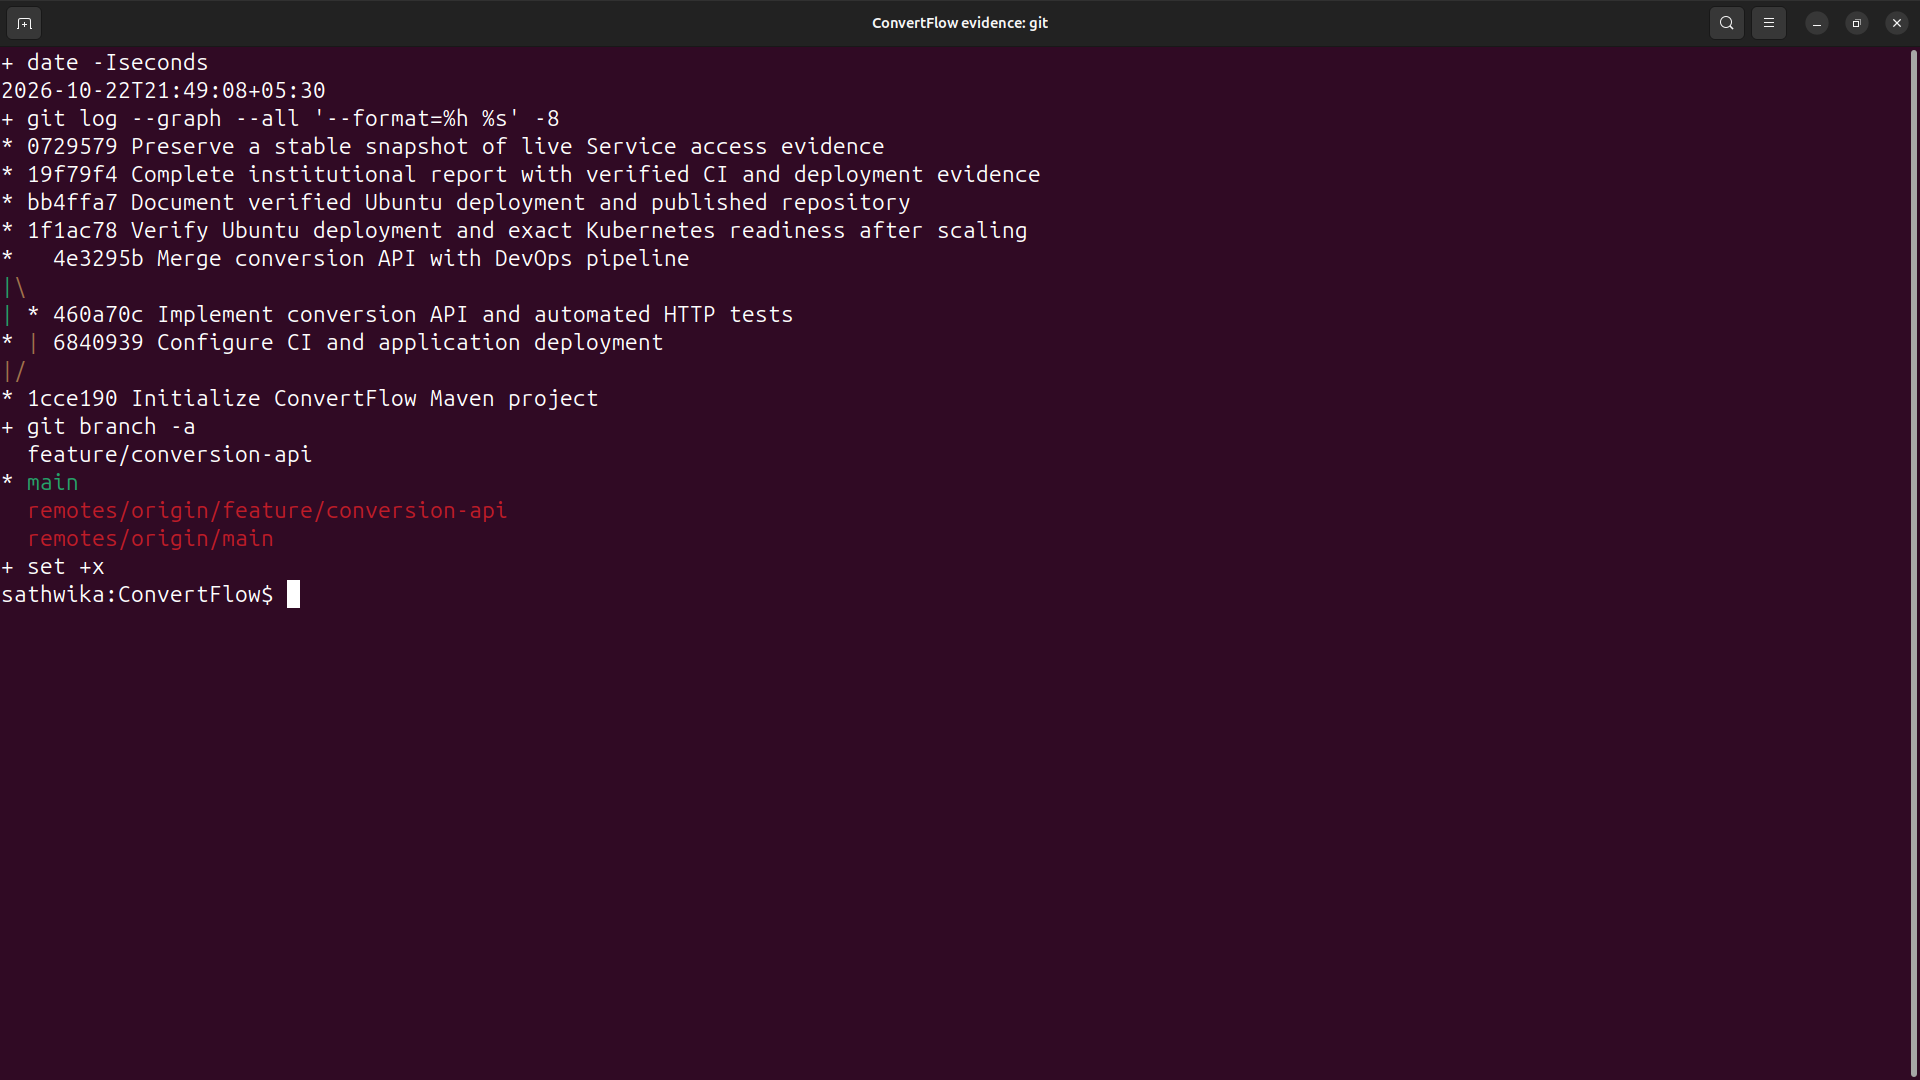
\includegraphics[width=\linewidth,height=0.78\textheight,keepaspectratio]{screenshots/terminal-git.png}\end{center}
Figure 1. GNOME Terminal: executed Git branch and merge history commands. The original feature branch and merge remain intact. Captured 22 Oct 2026, 21:49:12 +0530.
\end{landscape}
\clearpage\begin{landscape}\begin{center}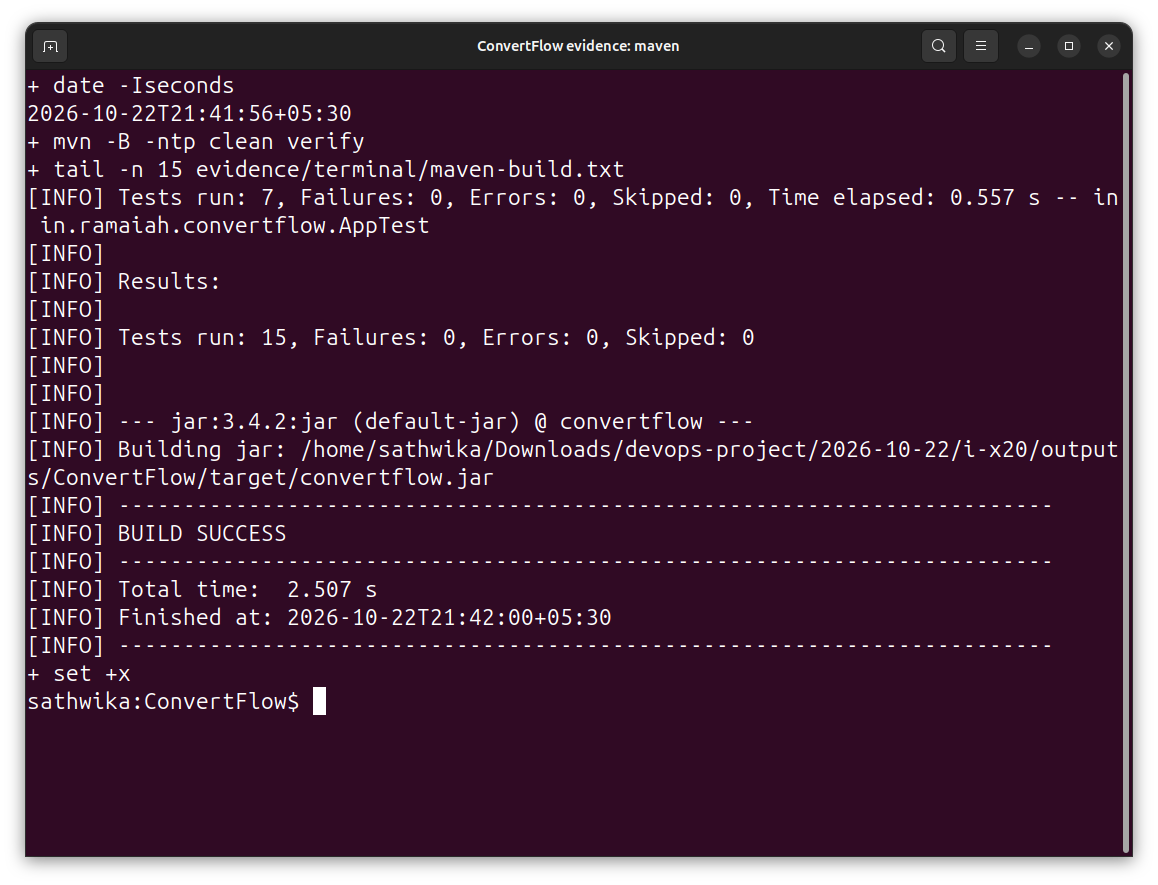
\includegraphics[width=\linewidth,height=0.78\textheight,keepaspectratio]{screenshots/terminal-maven.png}\end{center}
Figure 2. GNOME Terminal: Maven clean verify was executed and its saved log tail shows BUILD SUCCESS and all 15 tests passing. Captured 22 Oct 2026, 21:42:04 +0530.
\end{landscape}
\clearpage\begin{landscape}\begin{center}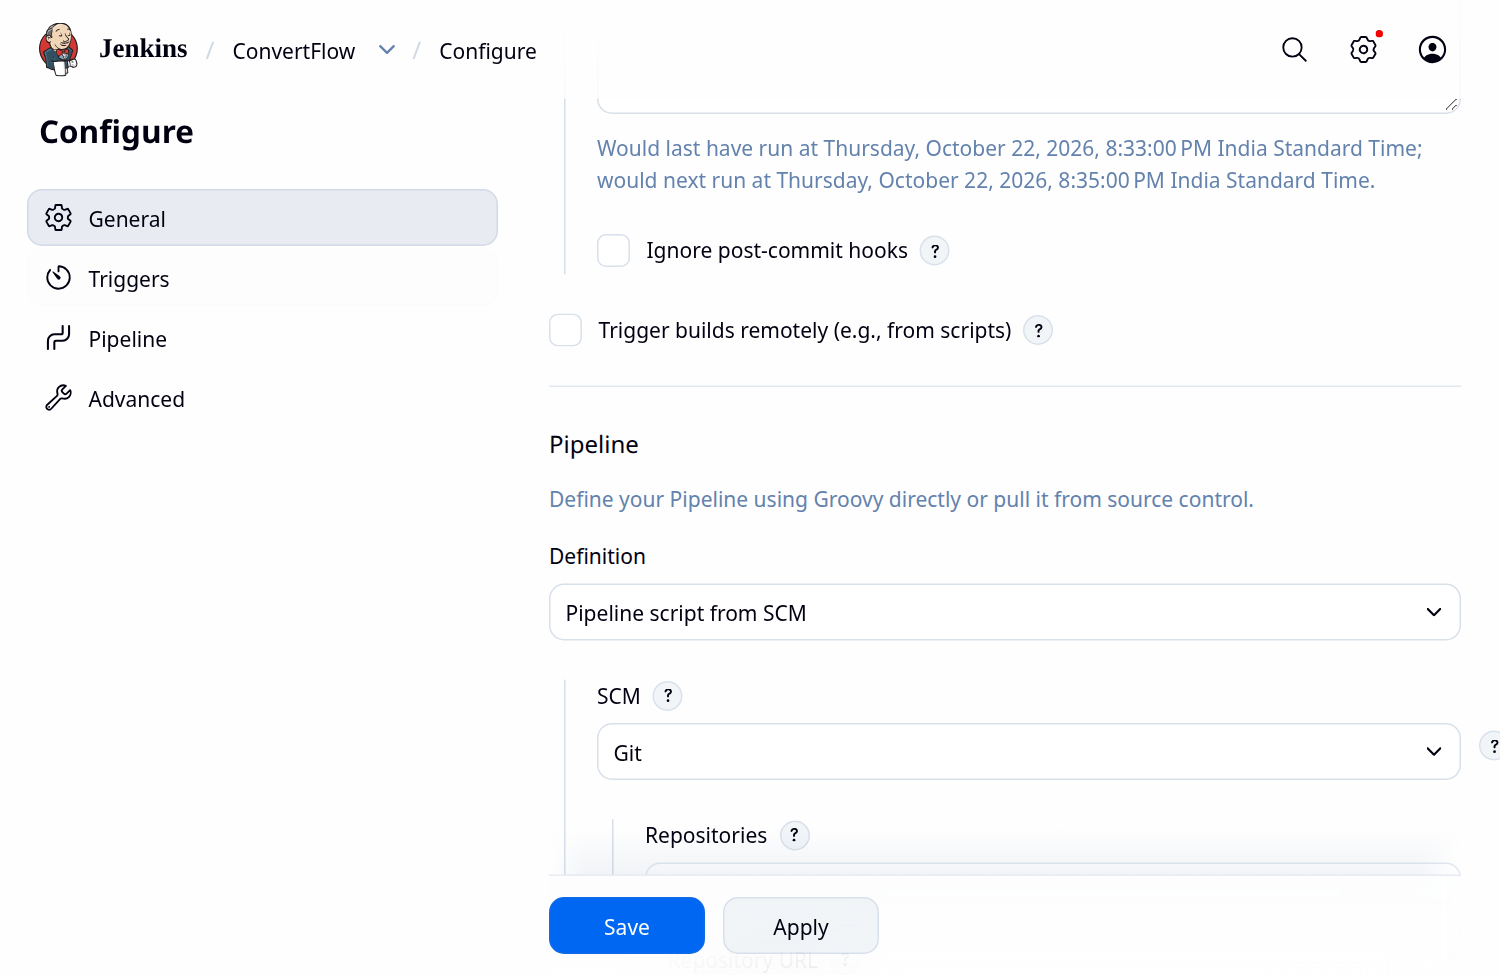
\includegraphics[width=\linewidth,height=0.78\textheight,keepaspectratio]{screenshots/ubuntu-jenkins-scm.png}\end{center}
Figure 3. Jenkins configuration: Pipeline script from SCM with Git selected.
\end{landscape}
\clearpage\begin{landscape}\begin{center}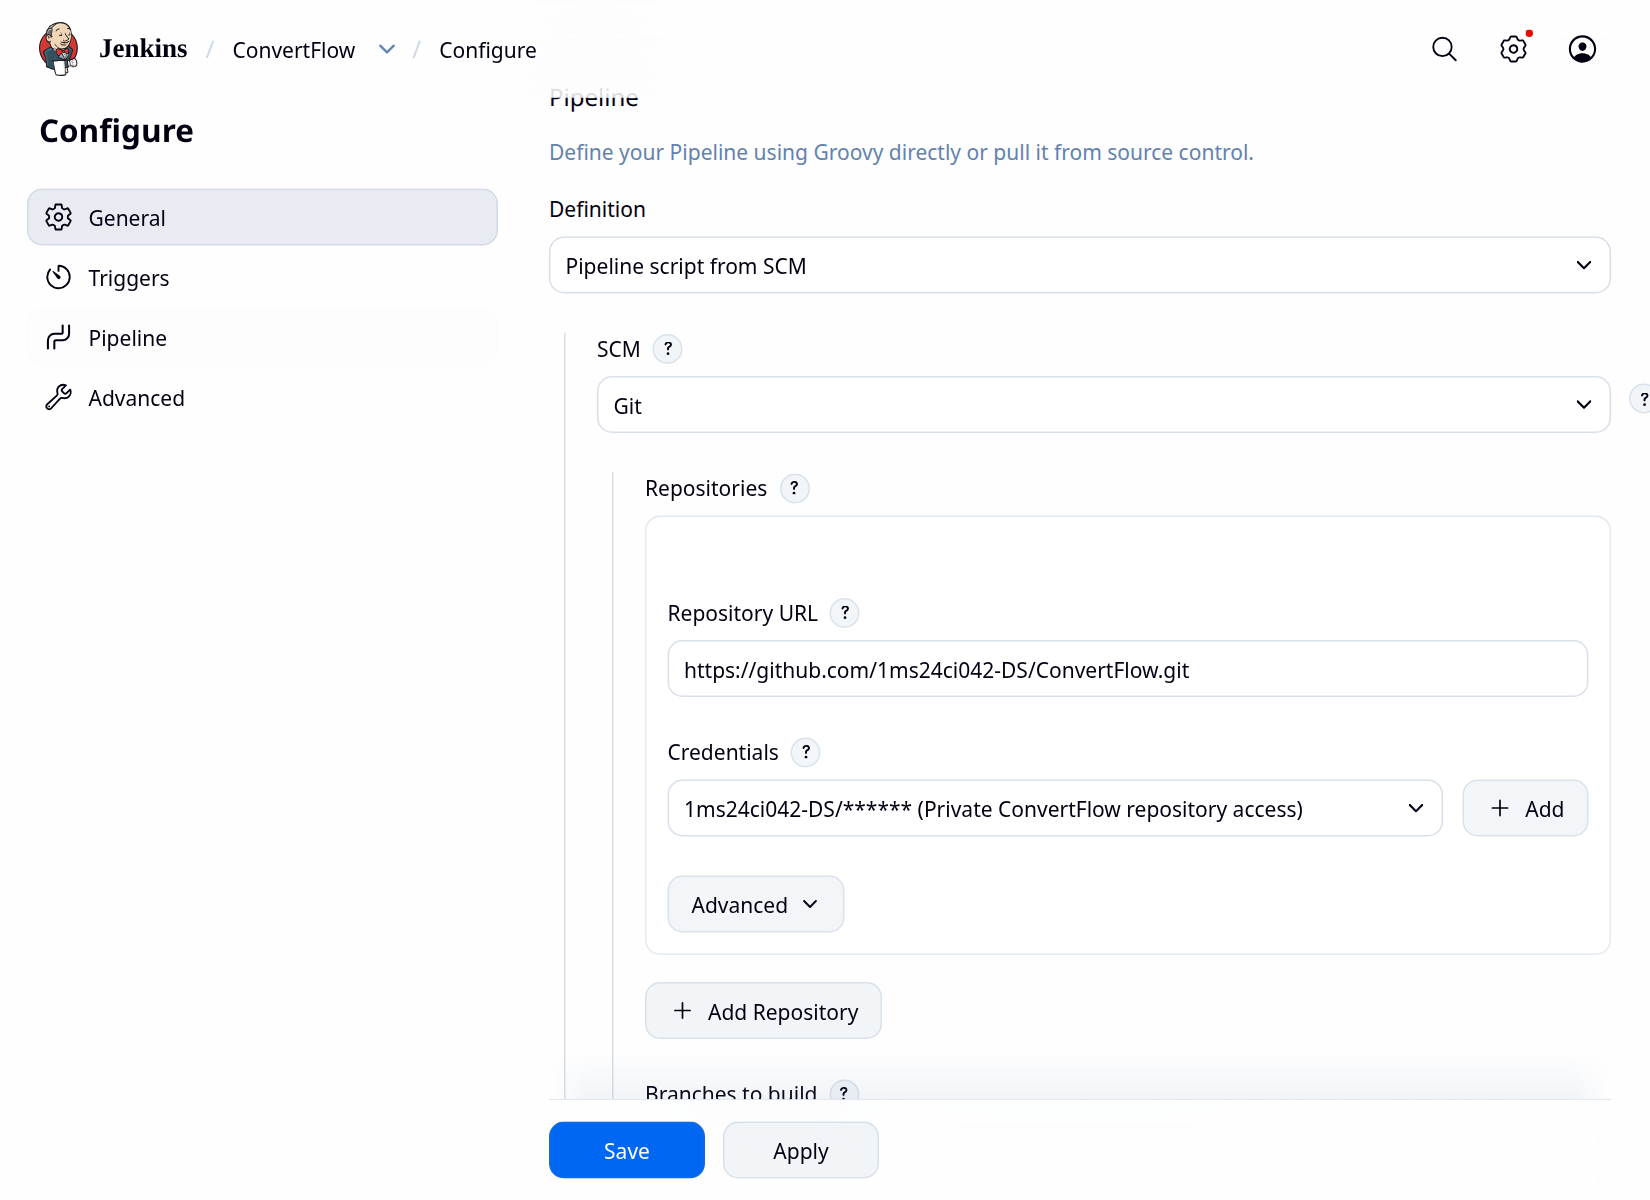
\includegraphics[width=\linewidth,height=0.78\textheight,keepaspectratio]{screenshots/ubuntu-jenkins-repository.png}\end{center}
Figure 4. Genuine Jenkins UI: actual private repository URL and credential identifier, without exposing a credential value.
\end{landscape}
\clearpage\begin{landscape}\begin{center}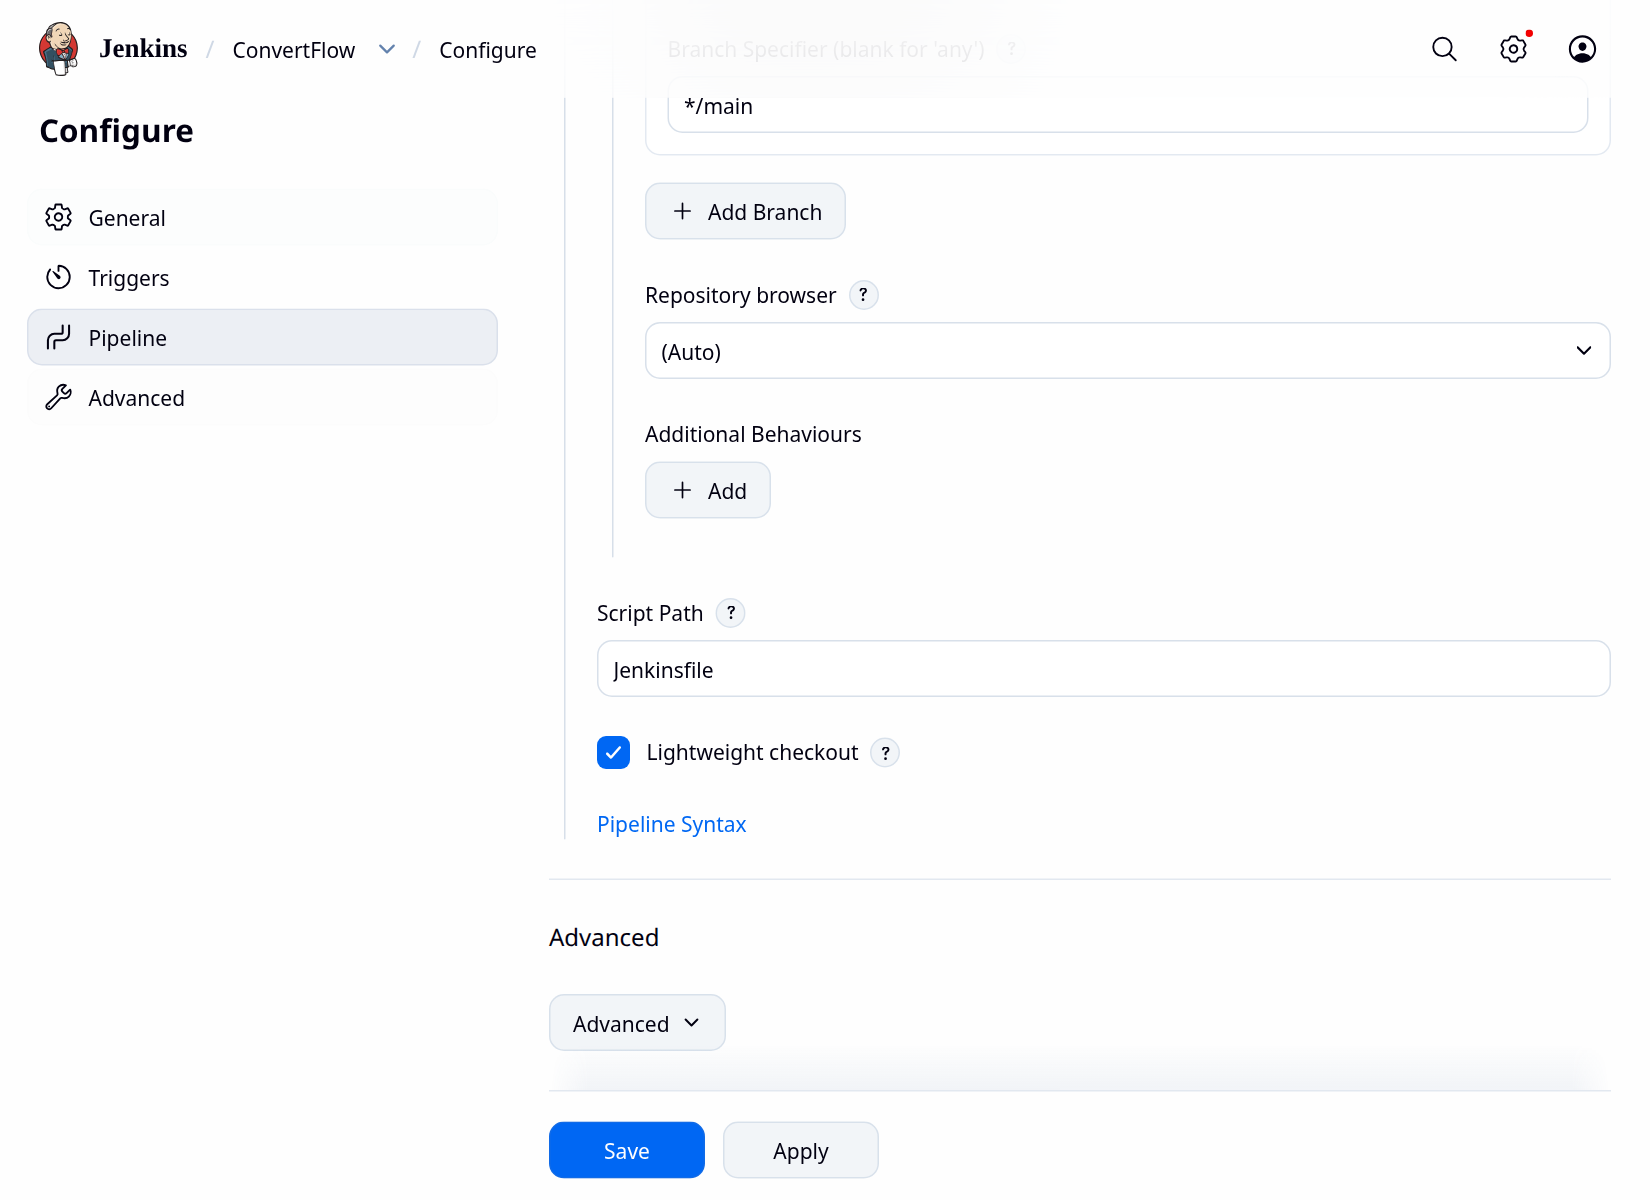
\includegraphics[width=\linewidth,height=0.78\textheight,keepaspectratio]{screenshots/ubuntu-jenkins-script-path.png}\end{center}
Figure 5. Genuine Jenkins UI: branch */main and Jenkinsfile script path; lightweight checkout is enabled.
\end{landscape}
\clearpage\begin{landscape}\begin{center}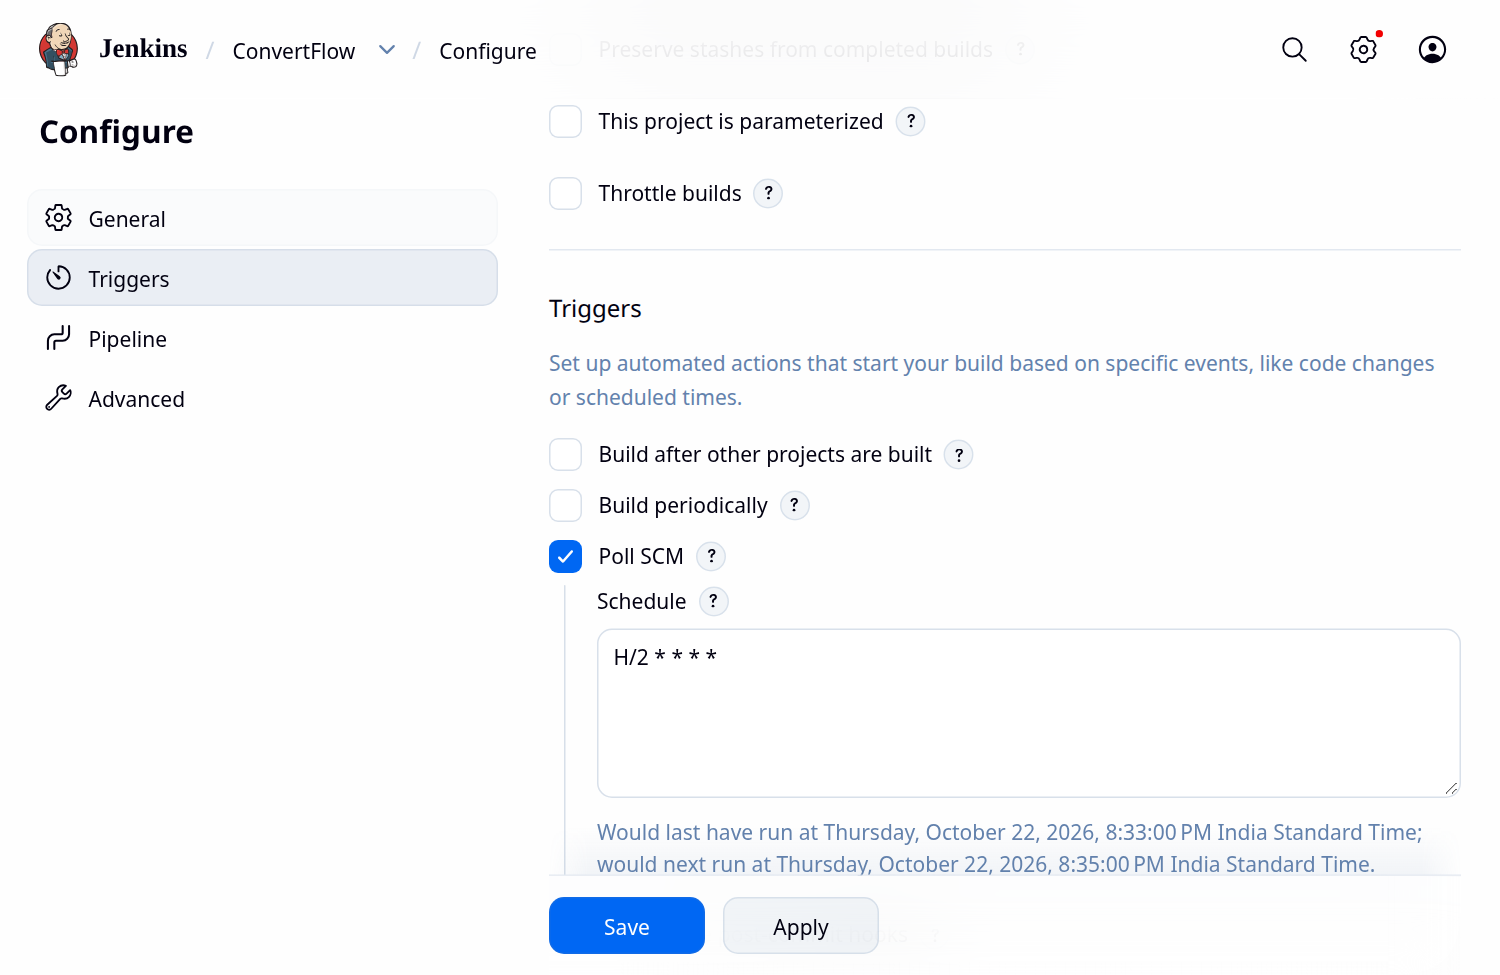
\includegraphics[width=\linewidth,height=0.78\textheight,keepaspectratio]{screenshots/ubuntu-jenkins-polling.png}\end{center}
Figure 6. Jenkins SCM polling configuration, using the two-minute schedule from Jenkinsfile.
\end{landscape}
\clearpage\begin{landscape}\begin{center}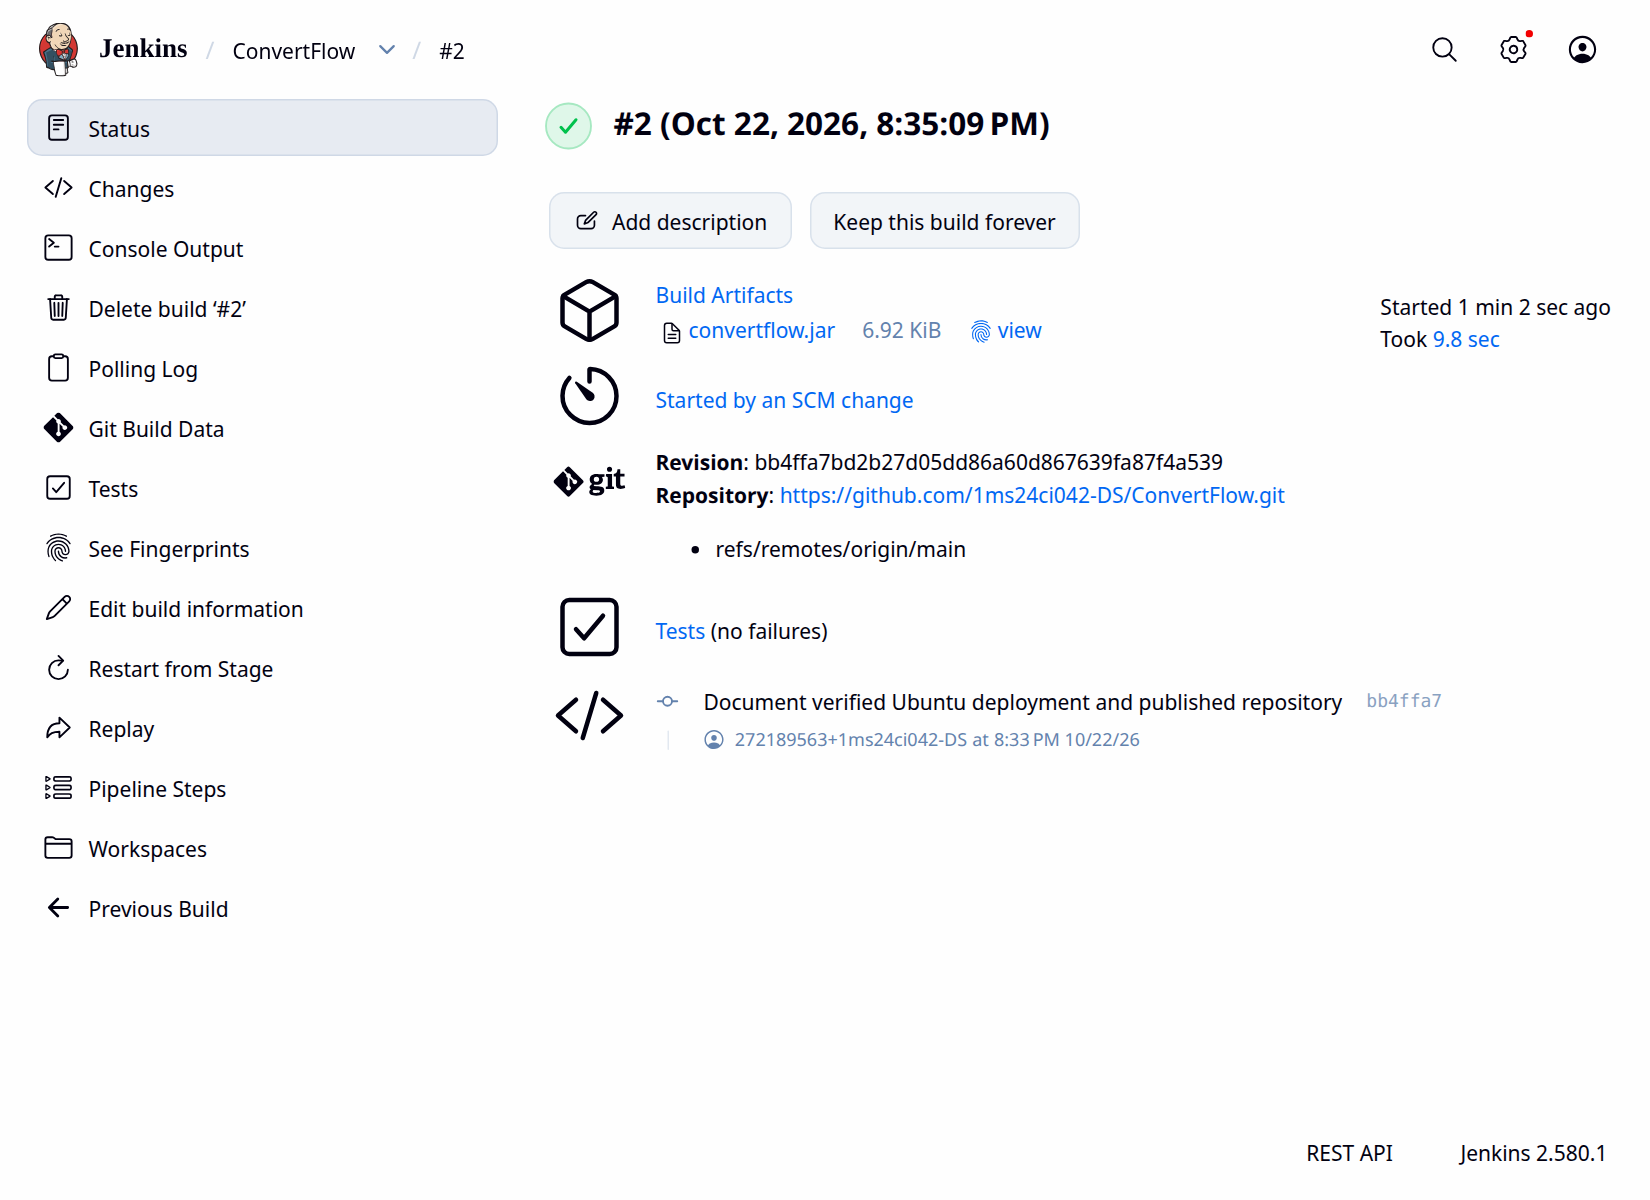
\includegraphics[width=\linewidth,height=0.78\textheight,keepaspectratio]{screenshots/ubuntu-jenkins-auto-build.png}\end{center}
Figure 7. Actual Jenkins build \#2 page showing the SCM change cause and archived convertflow.jar.
\end{landscape}
\clearpage\begin{landscape}\begin{center}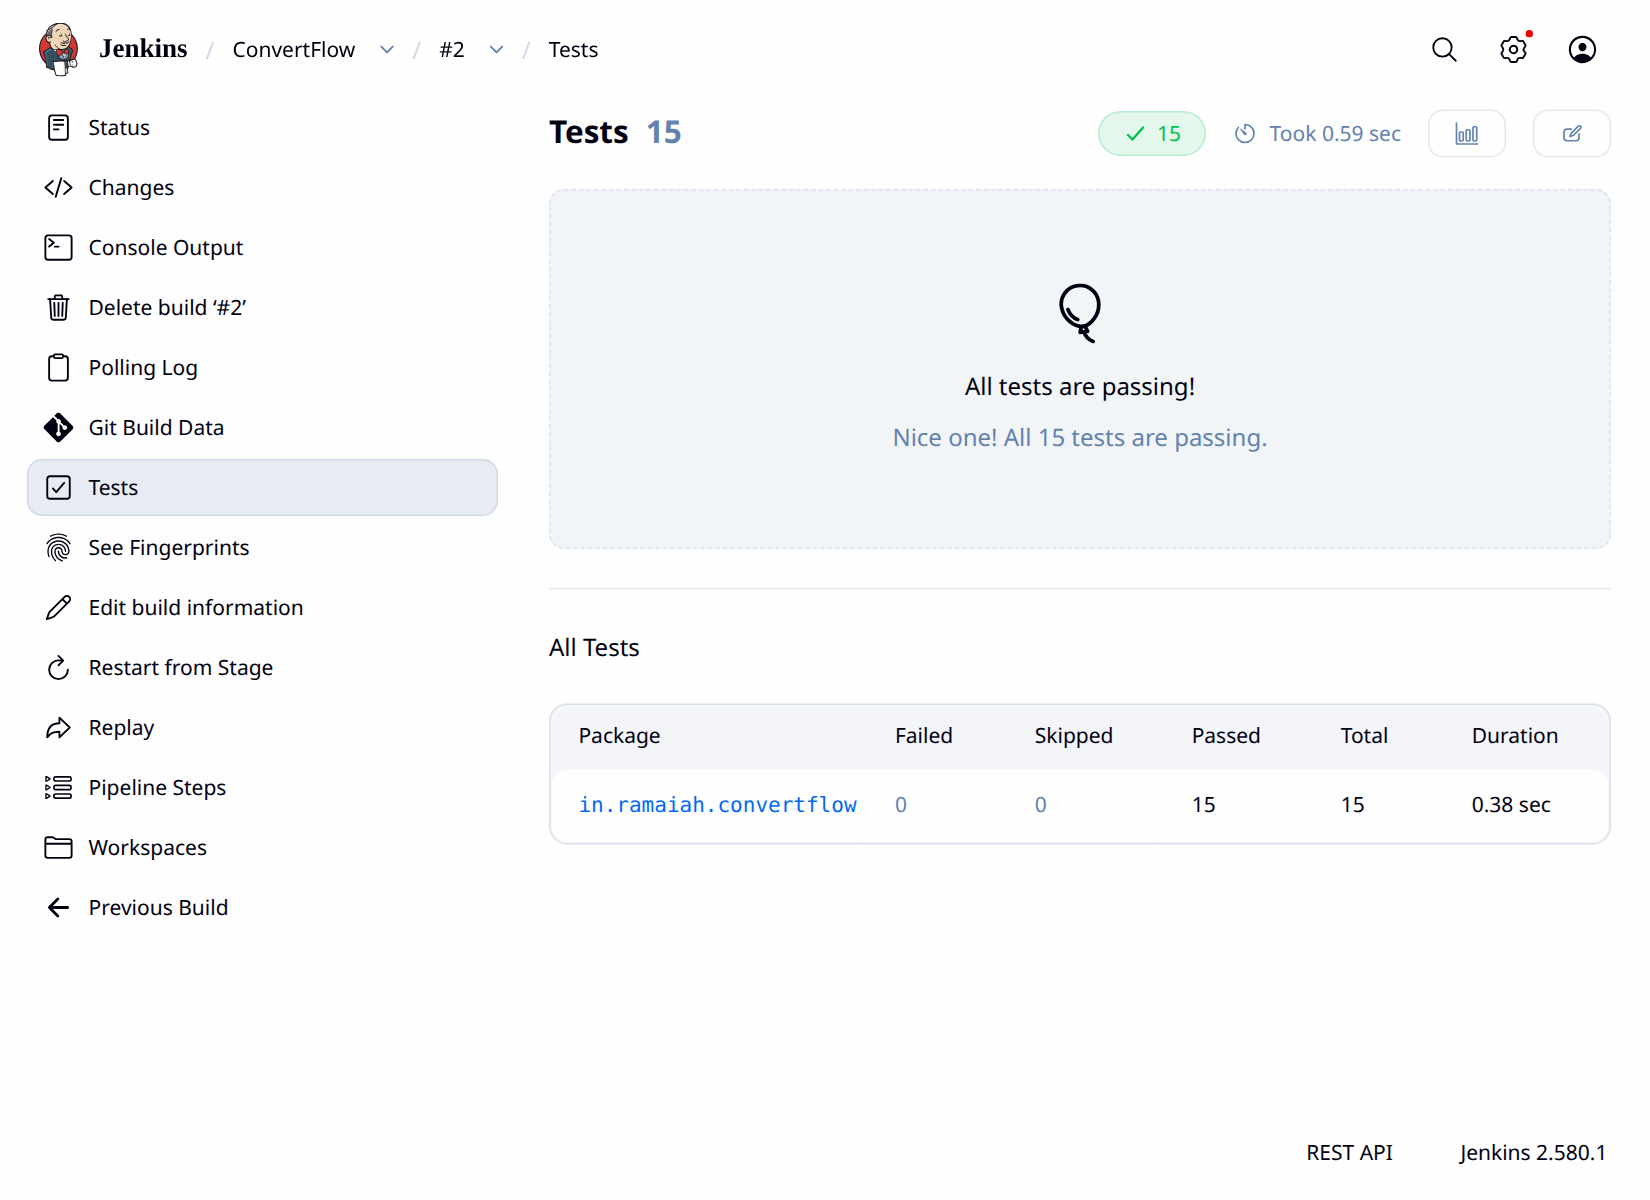
\includegraphics[width=\linewidth,height=0.78\textheight,keepaspectratio]{screenshots/ubuntu-jenkins-auto-tests.png}\end{center}
Figure 8. Actual Jenkins JUnit report for the automatic build: all 15 tests passed.
\end{landscape}
\clearpage\begin{landscape}\begin{center}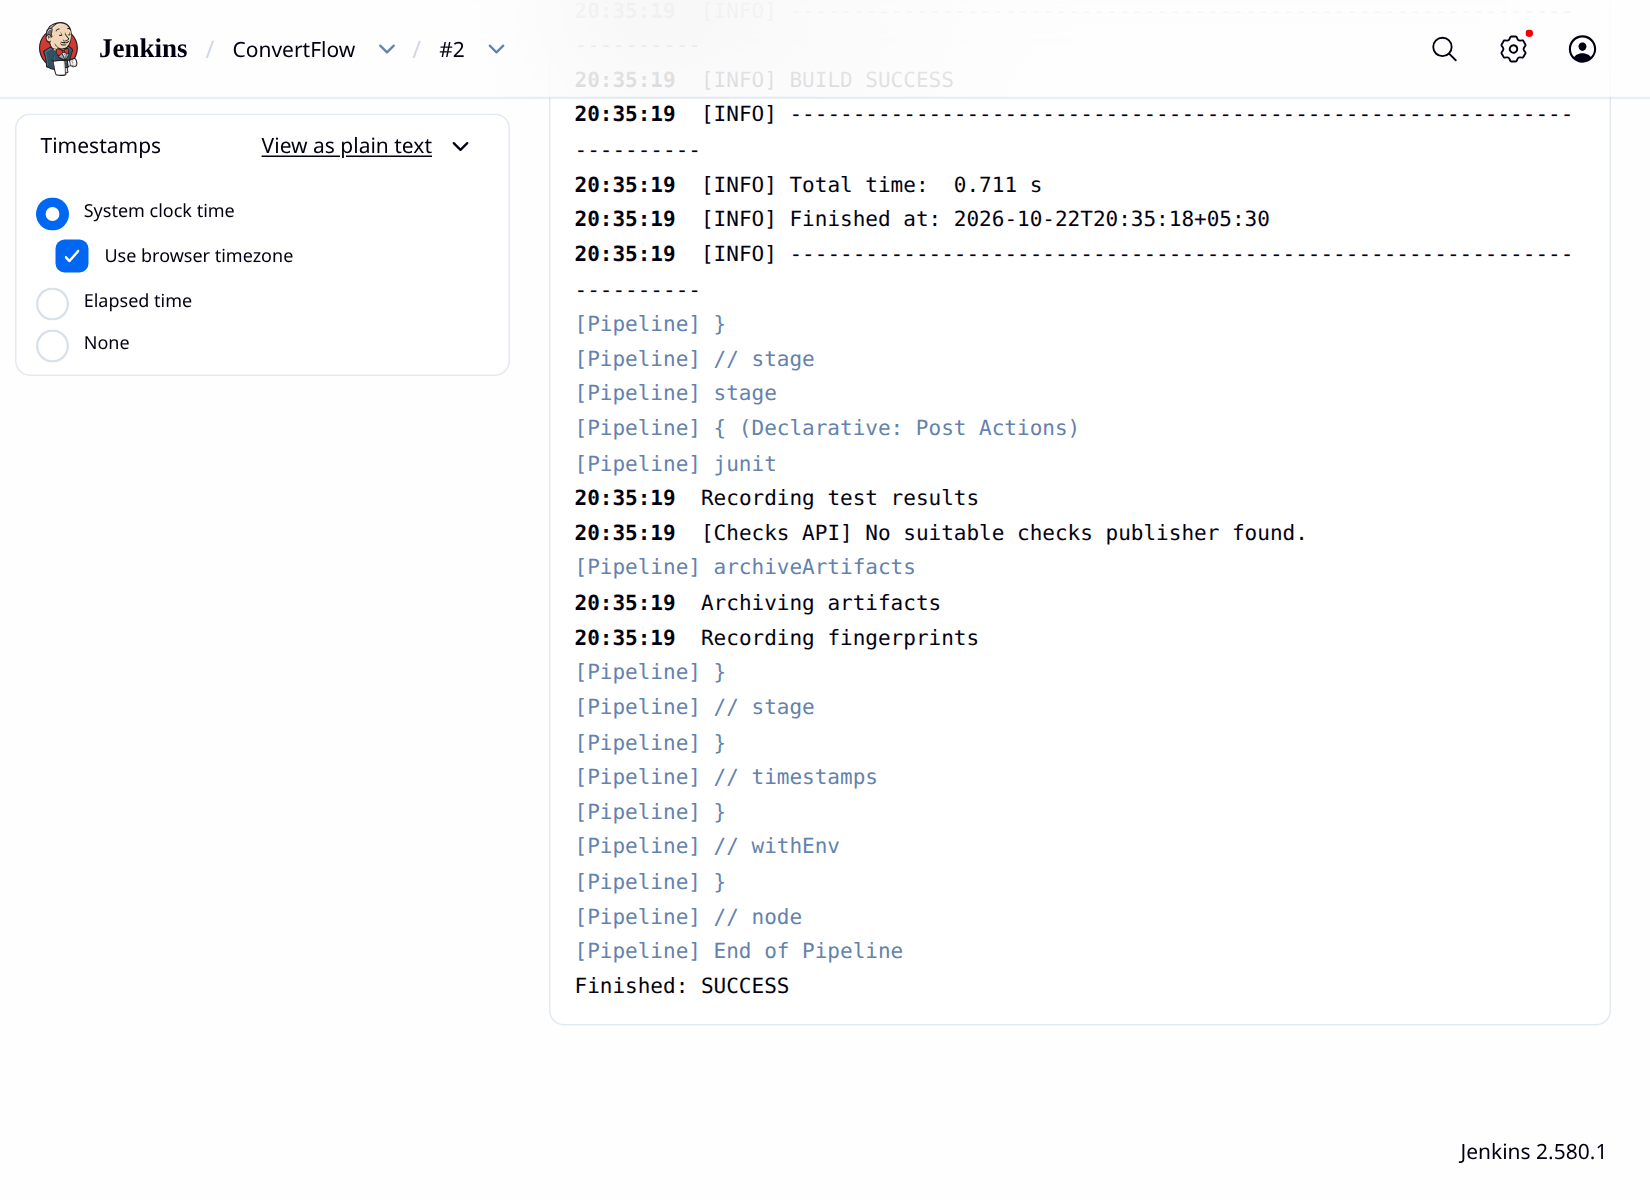
\includegraphics[width=\linewidth,height=0.78\textheight,keepaspectratio]{screenshots/ubuntu-jenkins-auto-console.png}\end{center}
Figure 9. Actual Jenkins console tail showing test-result publication, artifact archival and SUCCESS.
\end{landscape}
The expected 5 km conversion is 3.1068559611866697 miles. Five packaged-service HTTP contract checks additionally verified health, length conversion, temperature conversion, incompatible dimensions and an unknown route. These results are recorded in host-api-checks.txt.

\subsection*{Conclusion}
The verified workflow connects a real GitHub push to a tested and archived artifact through Jenkins SCM polling. The build cause and revision establish that the automatic run used the new commit. Separating tests from packaging makes the failure gate visible, while JUnit results and fingerprints make the output reviewable.

\subsection*{References}
Apache Maven: Build Lifecycle: https://maven.apache.org/guides/introduction/introduction-to-the-lifecycle.html (accessed 22 October 2026).

Jenkins: Pipeline Syntax: https://www.jenkins.io/doc/book/pipeline/syntax/ (accessed 22 October 2026).

Git: merge documentation: https://git-scm.com/docs/git-merge (accessed 22 October 2026).

Project repository: https://github.com/1ms24ci042-DS/ConvertFlow (accessed 22 October 2026).

\newpage
\section*{Component 2: Configuration Management with Ansible and Deployment on Kubernetes}
\subsection*{Abstract}
The same application is deployed to this Ubuntu system using an Ansible role and systemd, and to a local Kind cluster using a multi-stage Docker image. Ansible was run twice with zero changes on the second run. The container and Kubernetes Service returned correct responses. Three Ready replicas were scaled to five and then back to three, with readiness and exact counts checked at every step.

\subsection*{Introduction}
Ansible expresses the host configuration as repeatable tasks, variables and change-triggered handlers. Docker packages the application runtime, and Kubernetes maintains the declared replica count and routes traffic through a Service. ConvertFlow is stateless, so replicas do not need shared storage. The deployment enhancement combines configuration injection and health checks, supported by a non-root multi-stage image.

\subsection*{Implementation}
\subsubsection*{Development Environment}
The target is the actual Ubuntu 24.04 laptop with systemd, ansible-core 2.16.3 and Docker Engine 29.1.3. Kind v0.27.0 runs a Kubernetes v1.32.2 node, matched to kubectl v1.32.2. Cached Linux x86\_64 binaries and the Jenkins WAR were checked against official SHA-256 values before use. The systemd app uses port 8080, Docker uses 8081, Jenkins uses 8082, and the Kubernetes Service is forwarded on 8083. The distinct ports allow all demonstrations to remain available.

\subsubsection*{Code}
The inventory targets localhost through a local connection. Privileged tasks were reviewed before execution. They install a Java runtime, create the convertflow service user and /opt/convertflow, copy the built JAR, and write /etc/systemd/system/convertflow.service. File changes notify Restart ConvertFlow; pending handlers run before the health check. app\_port, app\_user, app\_dir and app\_jar are role variables.

ansible/playbook.yml

\lstinputlisting{../ansible/playbook.yml}
ansible/roles/convertflow/defaults/main.yml

\lstinputlisting{../ansible/roles/convertflow/defaults/main.yml}
ansible/roles/convertflow/handlers/main.yml

\lstinputlisting{../ansible/roles/convertflow/handlers/main.yml}
The systemd unit runs /usr/bin/java as the unprivileged convertflow user, restarts on failure, and enables NoNewPrivileges, ProtectSystem, ProtectHome and PrivateTmp. scripts/deploy-ubuntu.sh checks port ownership before replacing the known manually launched app with the service and runs the playbook twice.

Dockerfile

\lstinputlisting{../Dockerfile}
The build stage runs Maven clean verify. The runtime stage copies only the executable JAR into a Java 17 runtime image and runs as UID/GID 10001. Docker inspection and an actual id command confirm the non-root identity. The full Kubernetes manifest is k8s/deployment.yaml; the following excerpt declares the ConfigMap and replica selector.

k8s/deployment.yaml (excerpt, lines 1-26)

\lstinputlisting[firstline=1,lastline=26]{../k8s/deployment.yaml}
\subsubsection*{Description}
The Docker image convertflow:1.0.0 was loaded into the named Kind cluster. The Deployment, its Pod template and the Service consistently select app=convertflow. The Service exposes 8080 with NodePort 30080; localhost:8083 is an active port-forward to that Service. EndpointSlice data confirms ready backend endpoints. scripts/deploy-kind.sh records 3 -> 5 -> 3; verify-replicas.py waits for the exact number of Ready Pods and no remaining terminating Pods, including after scale-down.

\subsection*{Enhancement with rationale}
Readiness and liveness HTTP probes request /health. Readiness determines eligibility to receive Service traffic; liveness detects an unhealthy running process and can trigger restart. The ConfigMap supplies APP\_PORT=8080, confirmed with printenv inside a live Pod. The multi-stage image excludes build tools from the runtime, and non-root settings reduce runtime privileges. These choices improve deployment consistency without introducing a database or extra service.

Live evidence verifies configured probes, healthy Ready Pods, configuration injection and successful Service traffic. Deliberate process failure or a probe-induced restart was not part of this demonstration, so no fault-recovery event is claimed. Scaling is manual, not autoscaling. /health reports JSON application status and does not implement Prometheus metrics.

\subsection*{Results}
Historical deployment on 22 October 2026 at approximately 20:26 IST: first run ok=9, changed=6, failed=0; original second run ok=8, changed=0, failed=0. The first-run transcript is preserved and displayed in a real terminal, clearly labelled as historical. During fresh verification, Maven rebuilt the JAR; a later Ansible run legitimately copied it and restarted the service (changed=2). The next unchanged run again reported ok=8, changed=0, failed=0. These fresh results and timestamps are recorded under evidence/terminal/. The active systemd service and health response are verified separately.

Kubernetes recorded three Ready Pods, then five Ready Pods, then exactly three Ready Pods with none terminating. The same ReplicaSet remained responsible for the scaled workload. The Service returned UP and the expected 5 km conversion result. Live ConfigMap, Pod, Deployment, Service, EndpointSlice and node details are included in evidence/live/.

\clearpage\begin{landscape}\begin{center}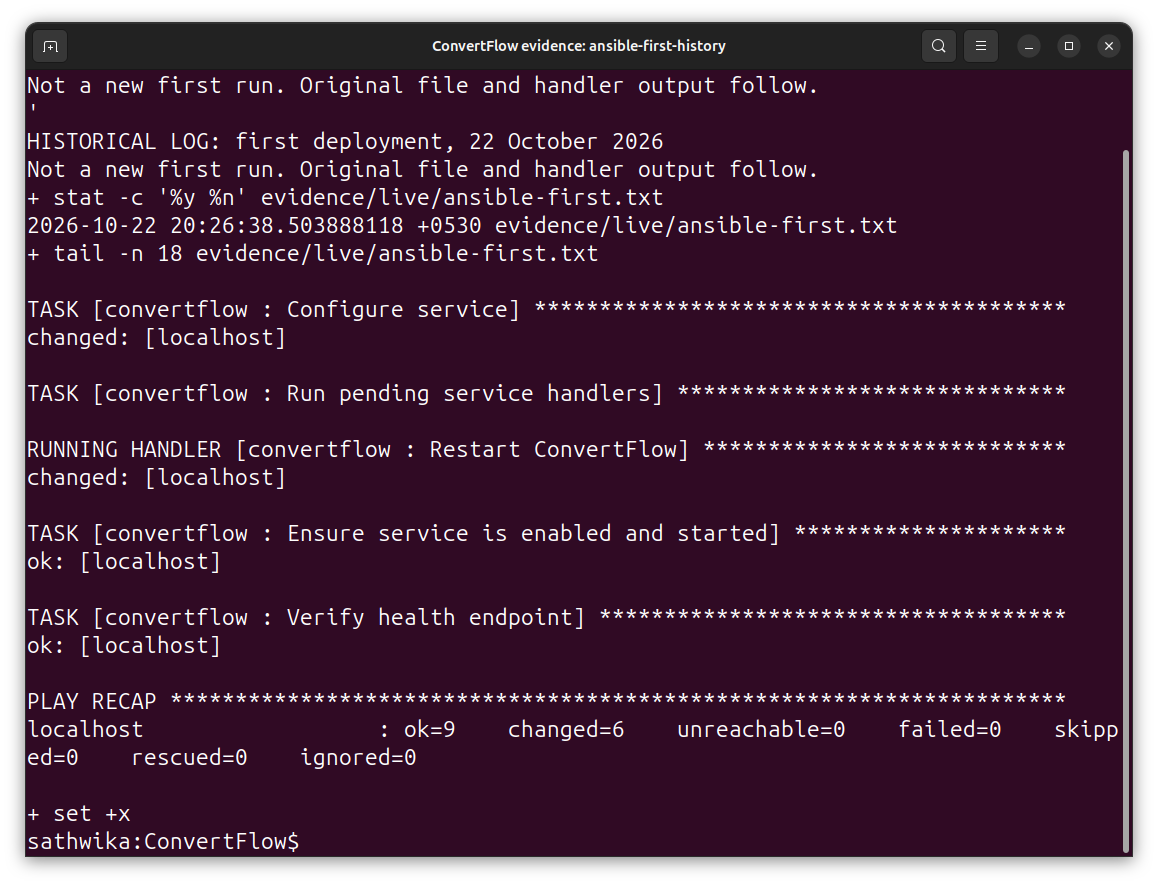
\includegraphics[width=\linewidth,height=0.78\textheight,keepaspectratio]{screenshots/terminal-ansible-first-history.png}\end{center}
Figure 10. GNOME Terminal reviewing the preserved FIRST-RUN log from 22 October 2026, approximately 20:26 IST: restart handler and changed=6. This is historical log review, not a newly executed first deployment. Captured 22 Oct 2026, 21:41:52 +0530.
\end{landscape}
\clearpage\begin{landscape}\begin{center}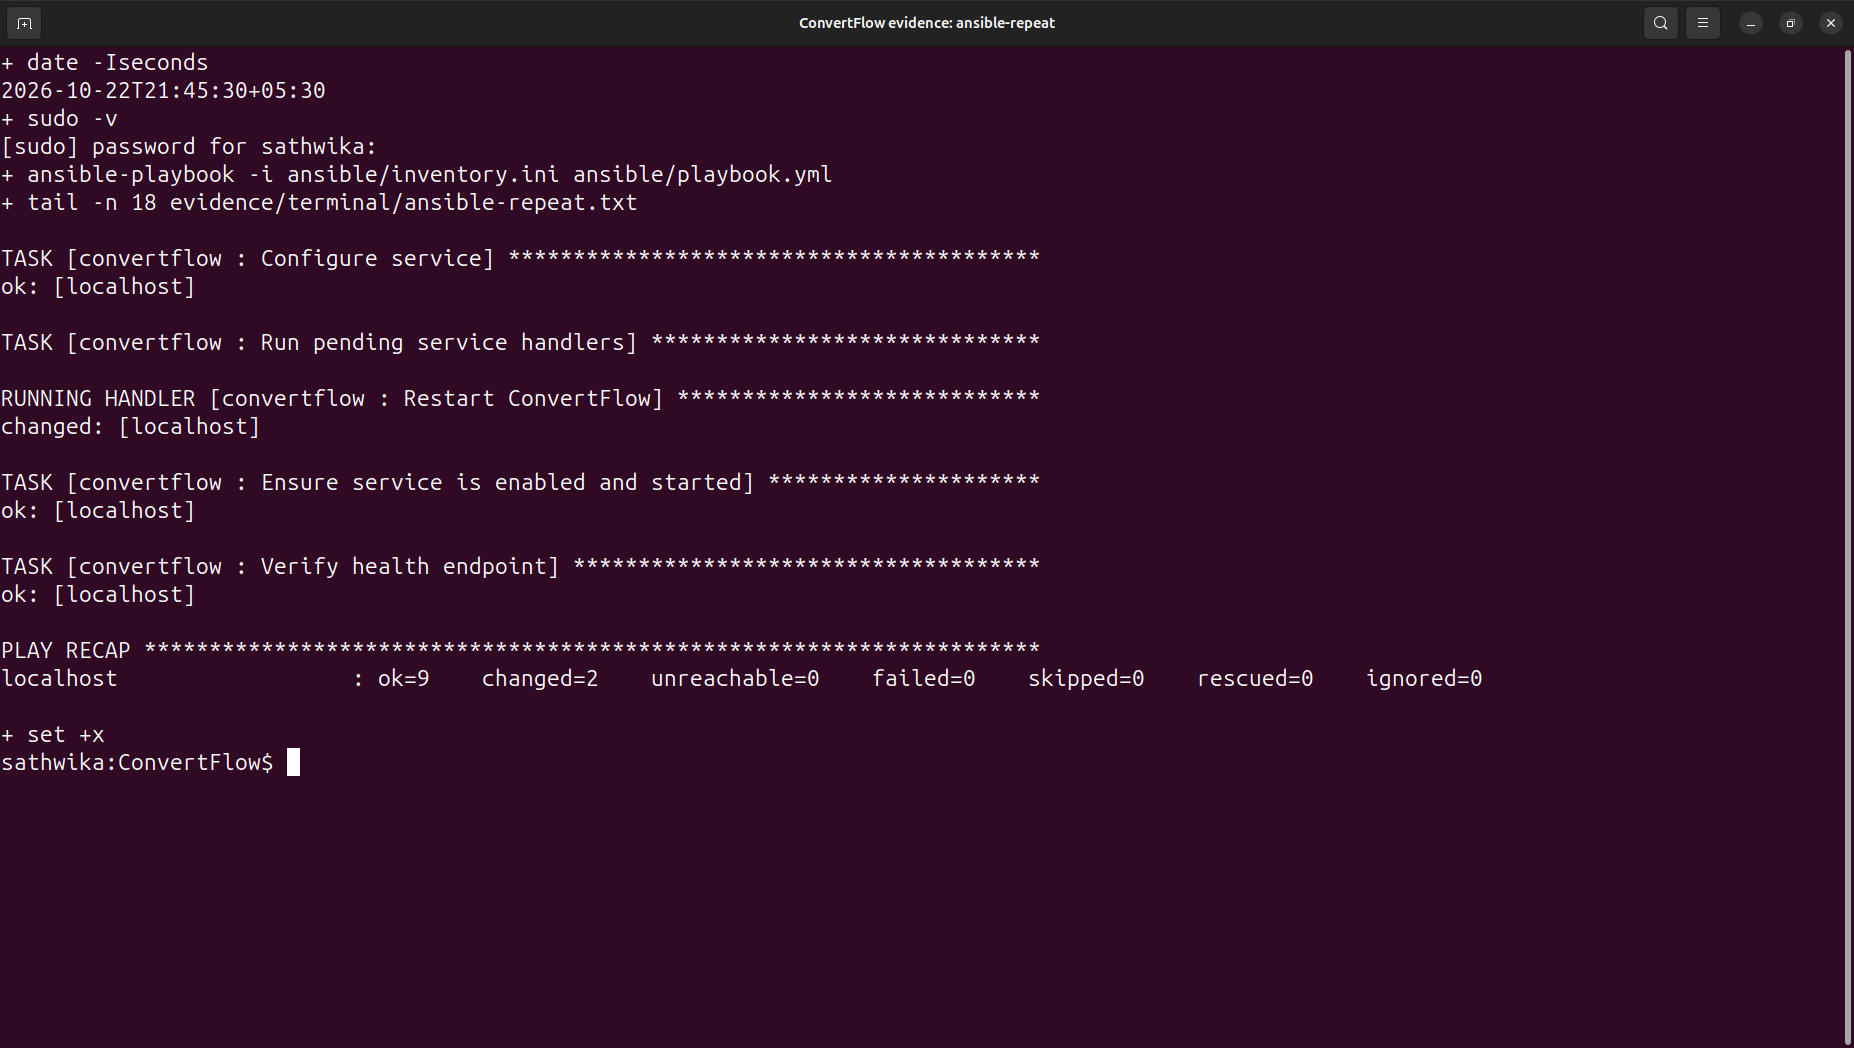
\includegraphics[width=\linewidth,height=0.78\textheight,keepaspectratio]{screenshots/terminal-ansible-refresh.png}\end{center}
Figure 11. GNOME Terminal: after Maven rebuilt the JAR, Ansible legitimately copied the new artifact and ran its restart handler; changed=2. No role or service setting was altered to manufacture changes. Captured 22 Oct 2026, 21:45:48 +0530.
\end{landscape}
\clearpage\begin{landscape}\begin{center}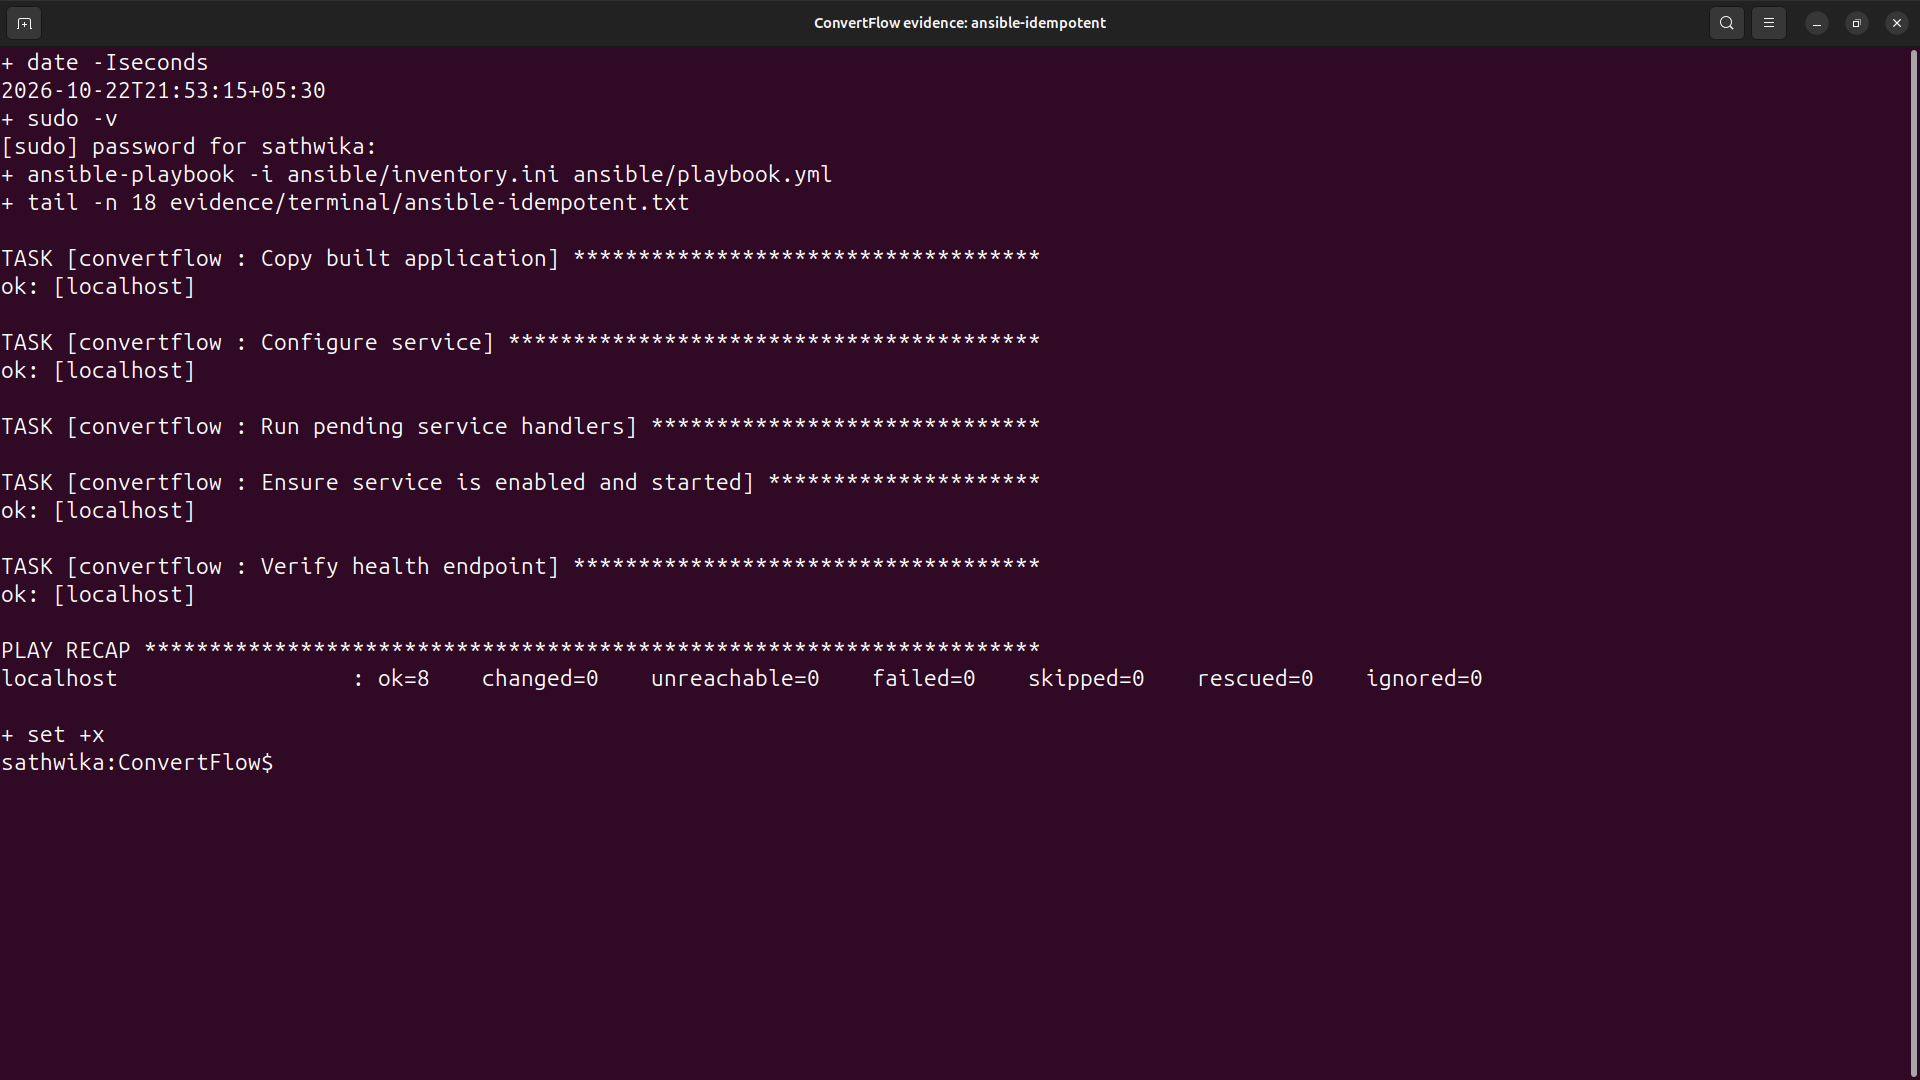
\includegraphics[width=\linewidth,height=0.78\textheight,keepaspectratio]{screenshots/terminal-ansible-idempotent.png}\end{center}
Figure 12. GNOME Terminal: the subsequent unchanged Ansible run shows ok=8, changed=0, failed=0; no restart handler executes. Captured 22 Oct 2026, 21:53:31 +0530.
\end{landscape}
\clearpage\begin{landscape}\begin{center}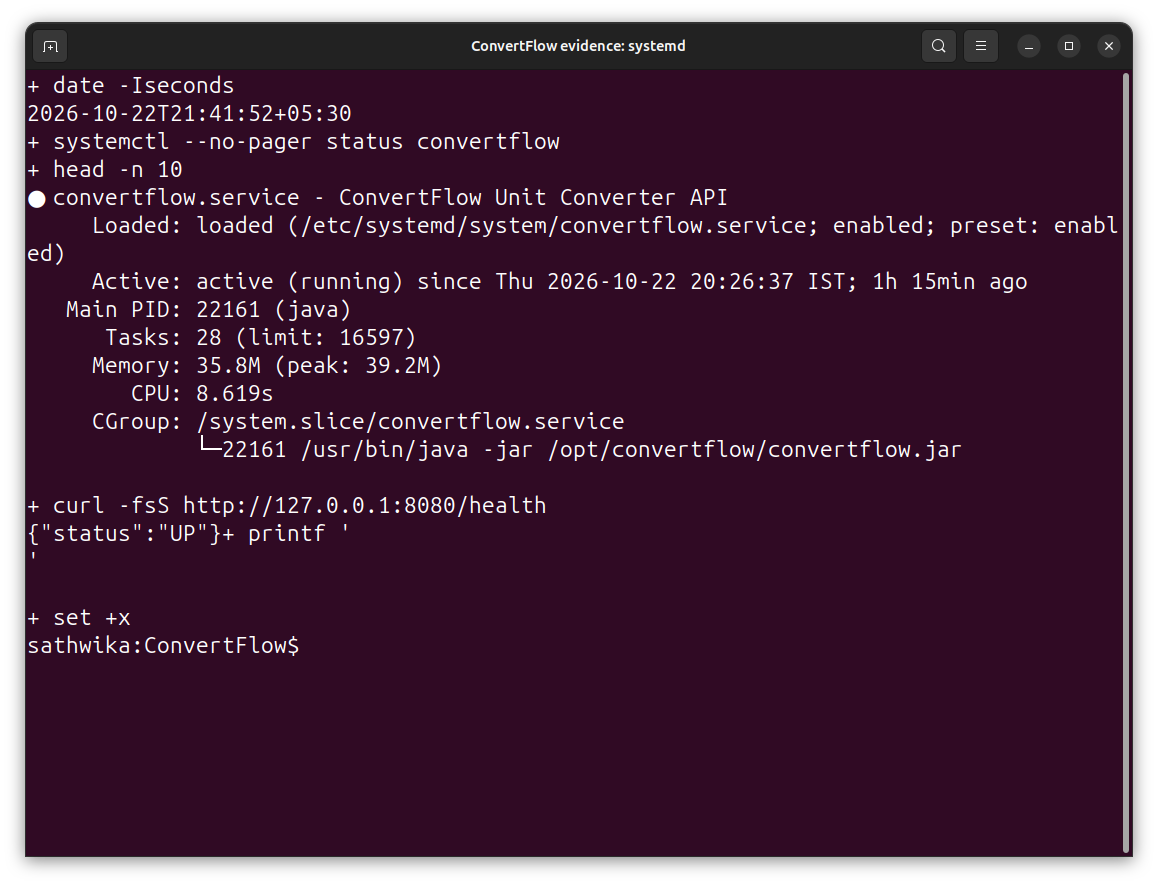
\includegraphics[width=\linewidth,height=0.78\textheight,keepaspectratio]{screenshots/terminal-systemd.png}\end{center}
Figure 13. GNOME Terminal: actual active systemd service and successful health response on port 8080. Captured 22 Oct 2026, 21:41:56 +0530.
\end{landscape}
\clearpage\begin{landscape}\begin{center}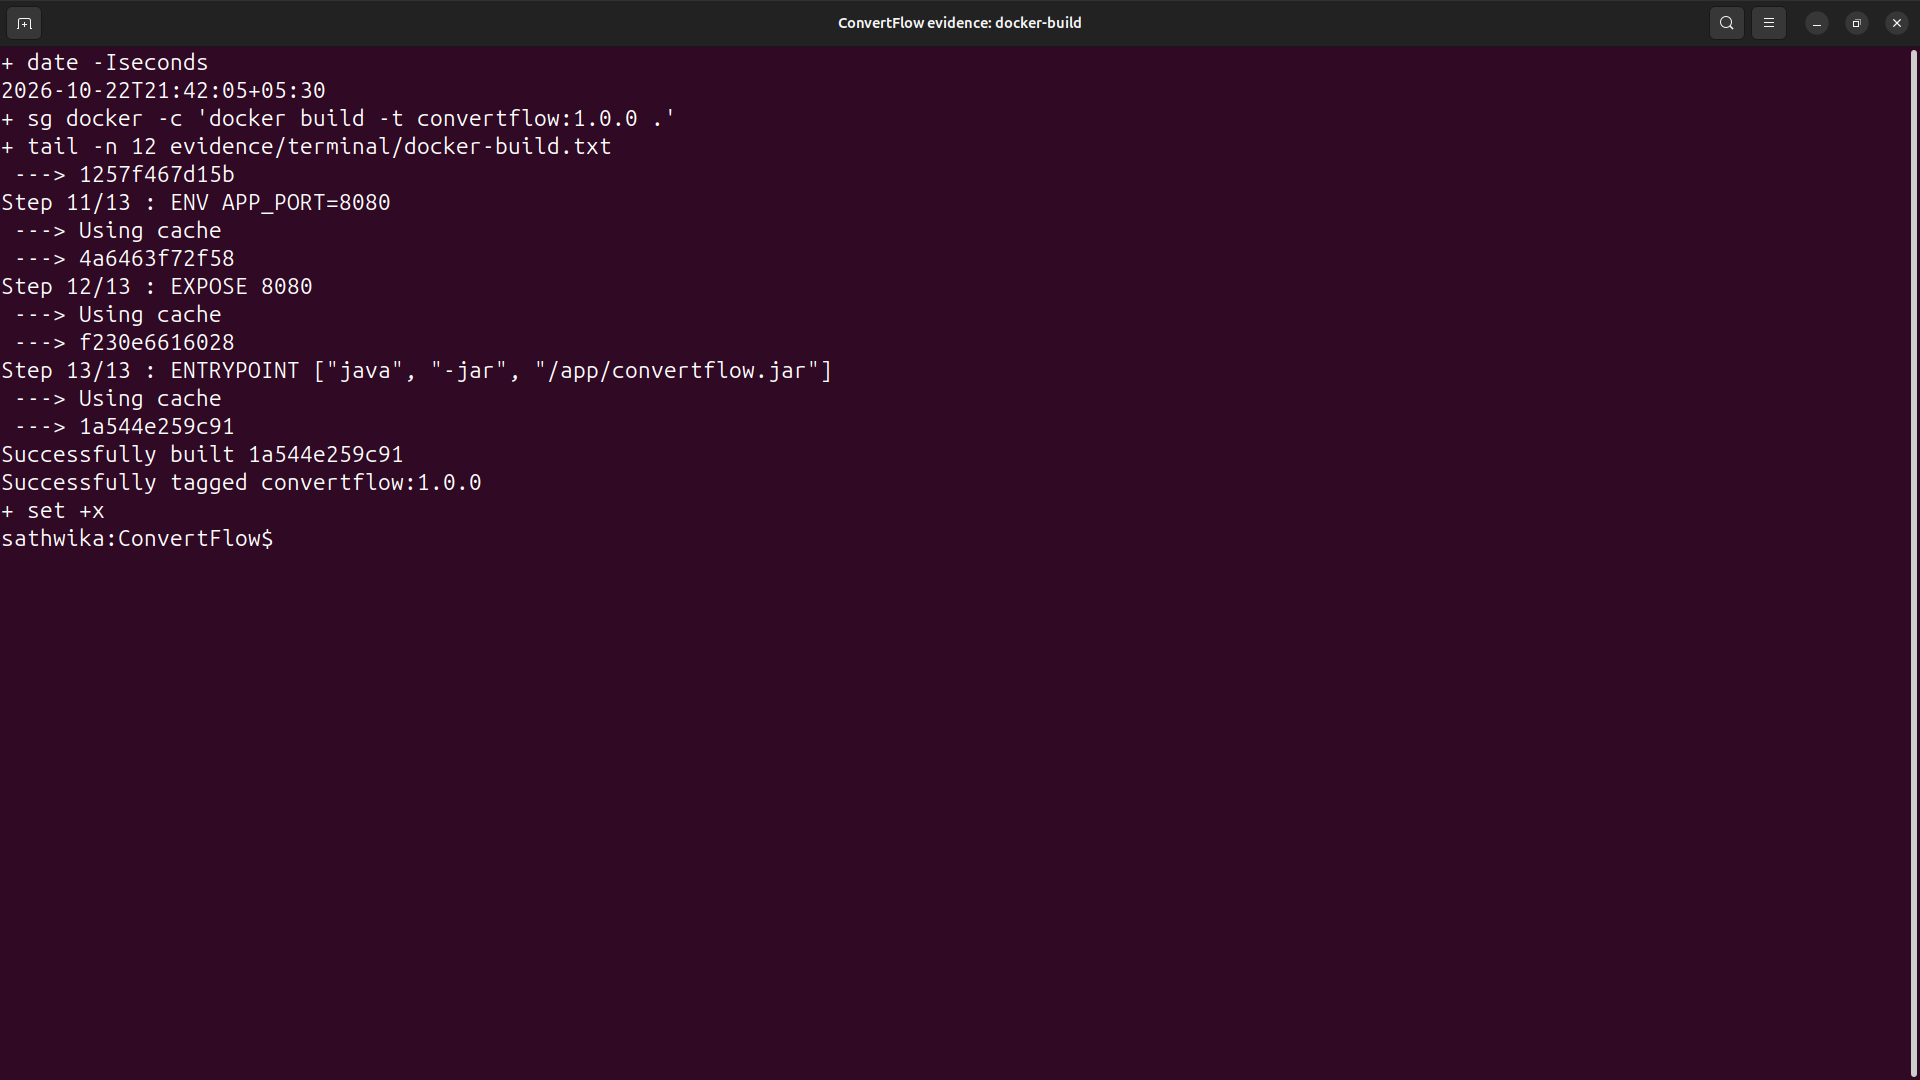
\includegraphics[width=\linewidth,height=0.78\textheight,keepaspectratio]{screenshots/terminal-docker-build.png}\end{center}
Figure 14. GNOME Terminal: the Docker image build was executed; its real log tail confirms the completed image and convertflow:1.0.0 tag. Captured 22 Oct 2026, 21:42:09 +0530.
\end{landscape}
\clearpage\begin{landscape}\begin{center}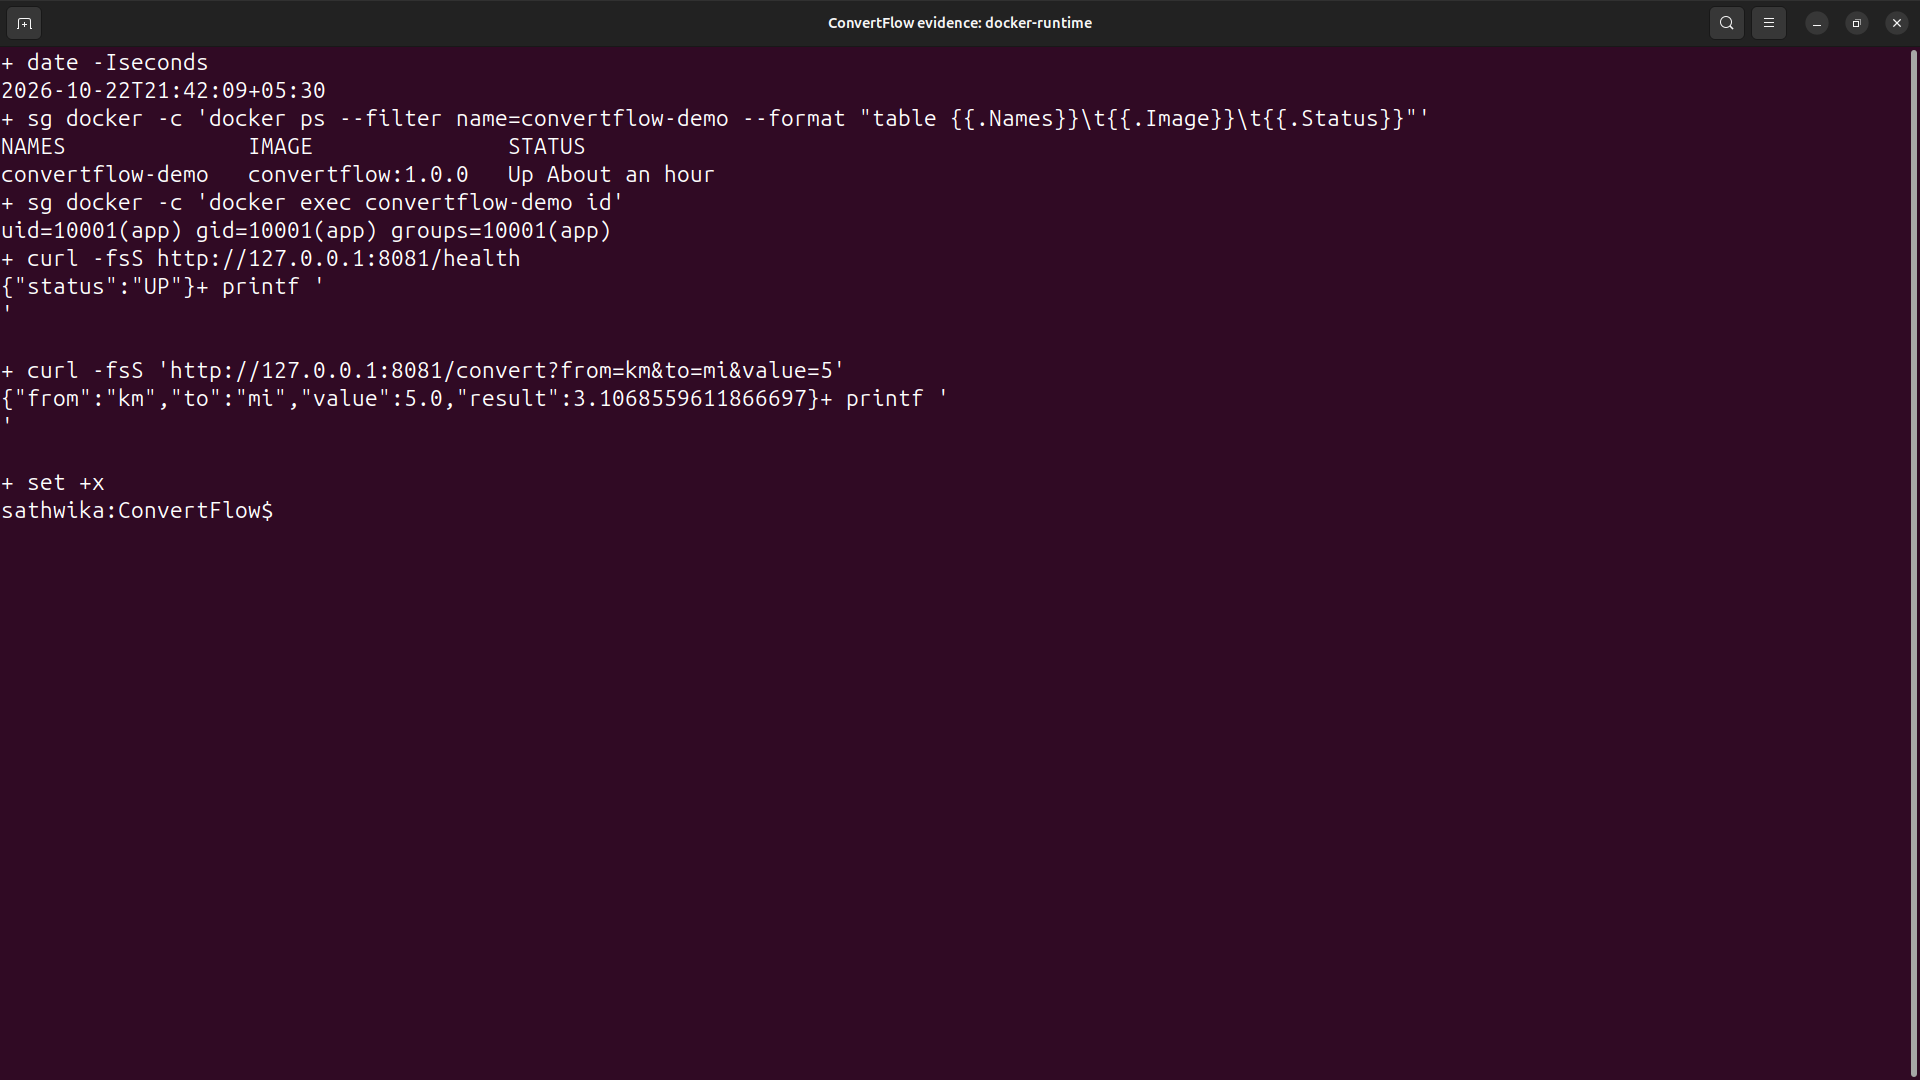
\includegraphics[width=\linewidth,height=0.78\textheight,keepaspectratio]{screenshots/terminal-docker-runtime.png}\end{center}
Figure 15. GNOME Terminal: running Docker container, non-root runtime identity, health response and correct conversion result on port 8081. Captured 22 Oct 2026, 21:42:13 +0530.
\end{landscape}
\clearpage\begin{landscape}\begin{center}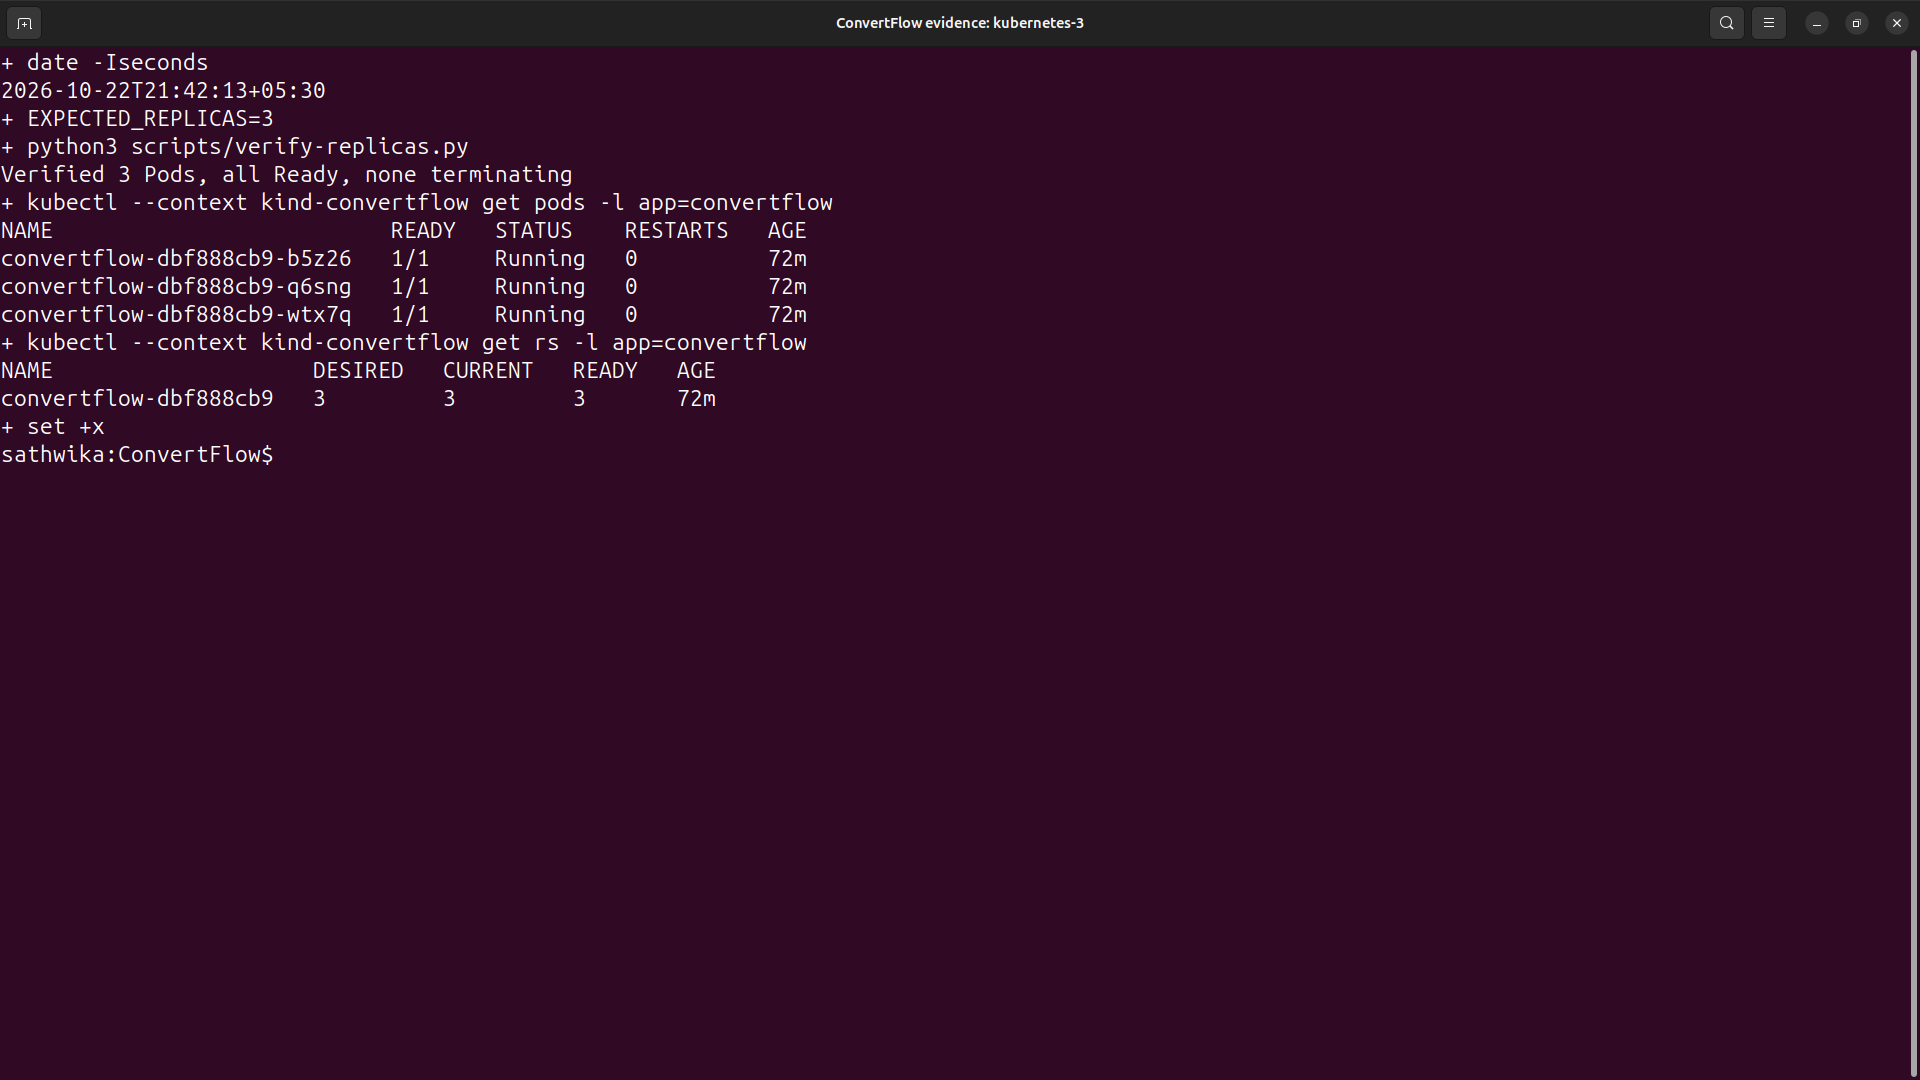
\includegraphics[width=\linewidth,height=0.78\textheight,keepaspectratio]{screenshots/terminal-kubernetes-3.png}\end{center}
Figure 16. GNOME Terminal: fresh verification of exactly three Ready Pods and the corresponding ReplicaSet before scaling. Captured 22 Oct 2026, 21:42:17 +0530.
\end{landscape}
\clearpage\begin{landscape}\begin{center}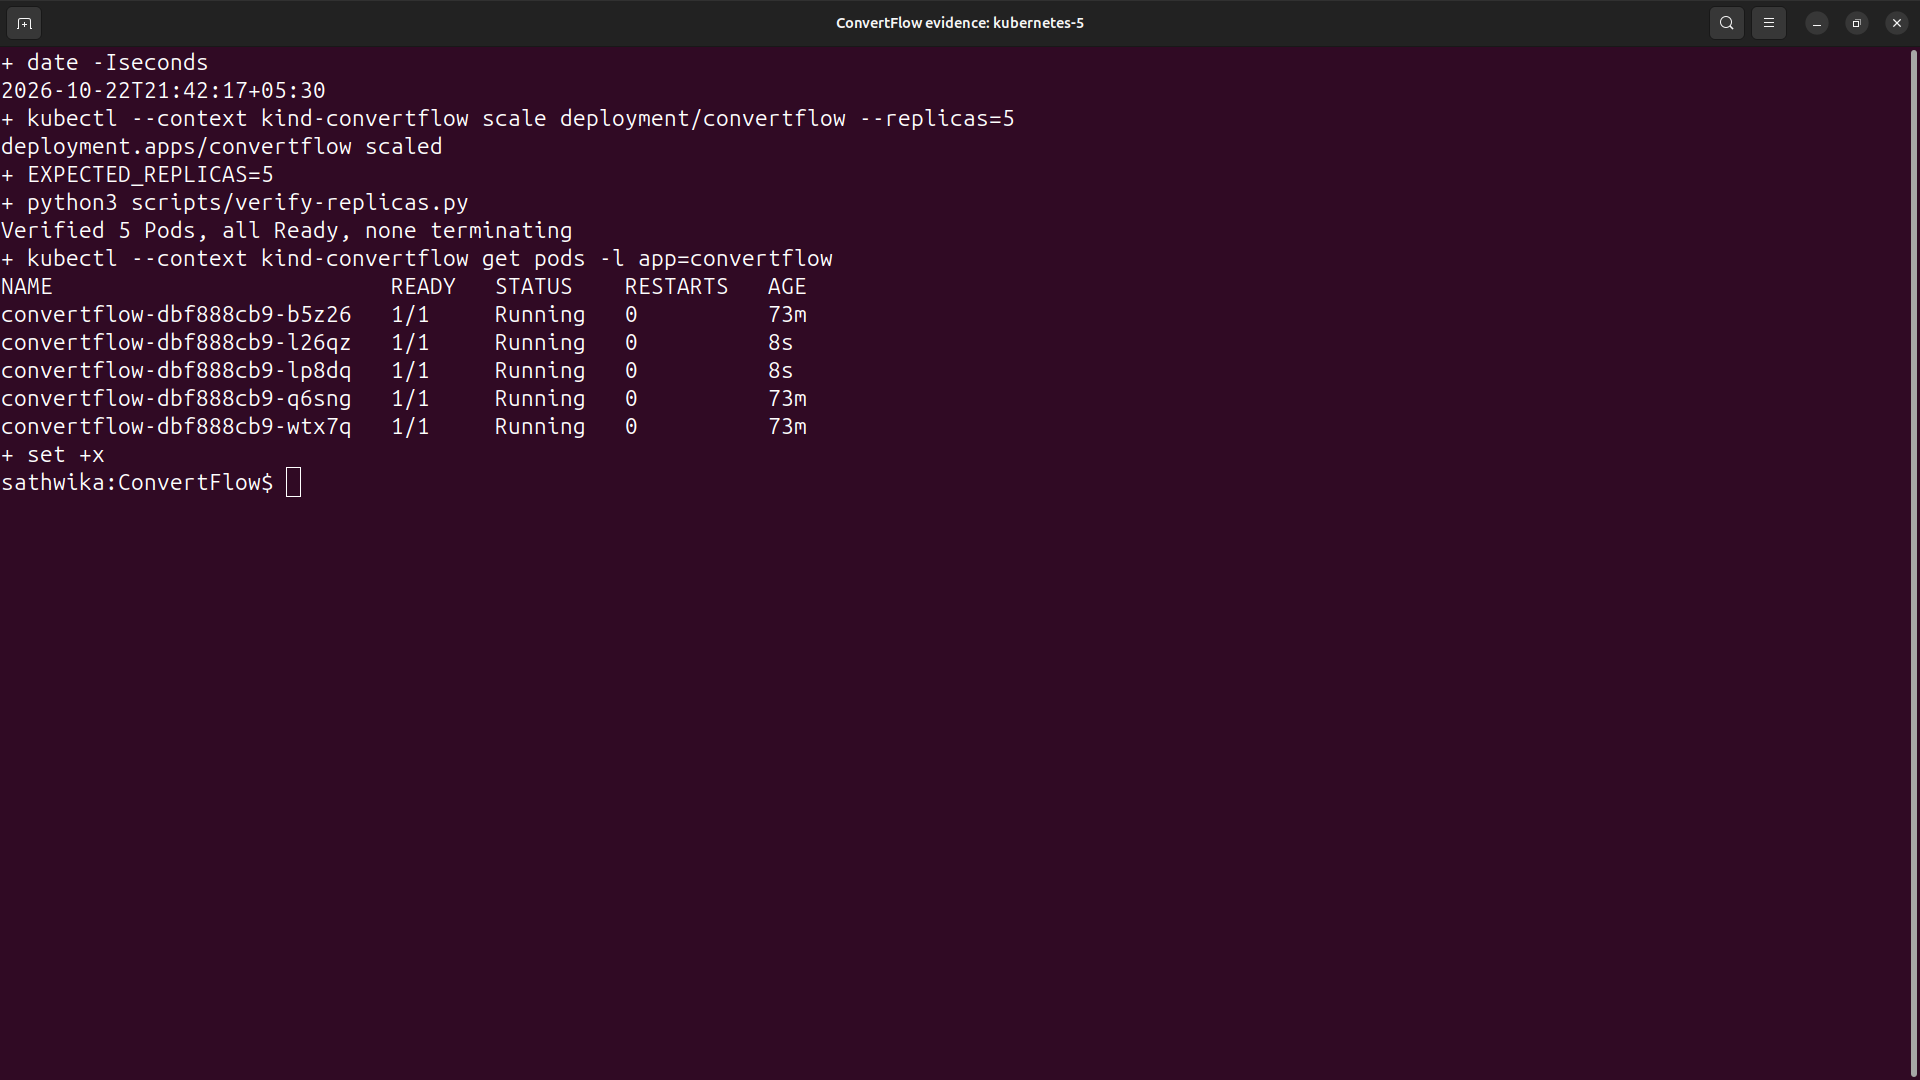
\includegraphics[width=\linewidth,height=0.78\textheight,keepaspectratio]{screenshots/terminal-kubernetes-5.png}\end{center}
Figure 17. GNOME Terminal: scale command to five replicas, exact readiness verification, and five Ready Pods. Captured 22 Oct 2026, 21:42:30 +0530.
\end{landscape}
\clearpage\begin{landscape}\begin{center}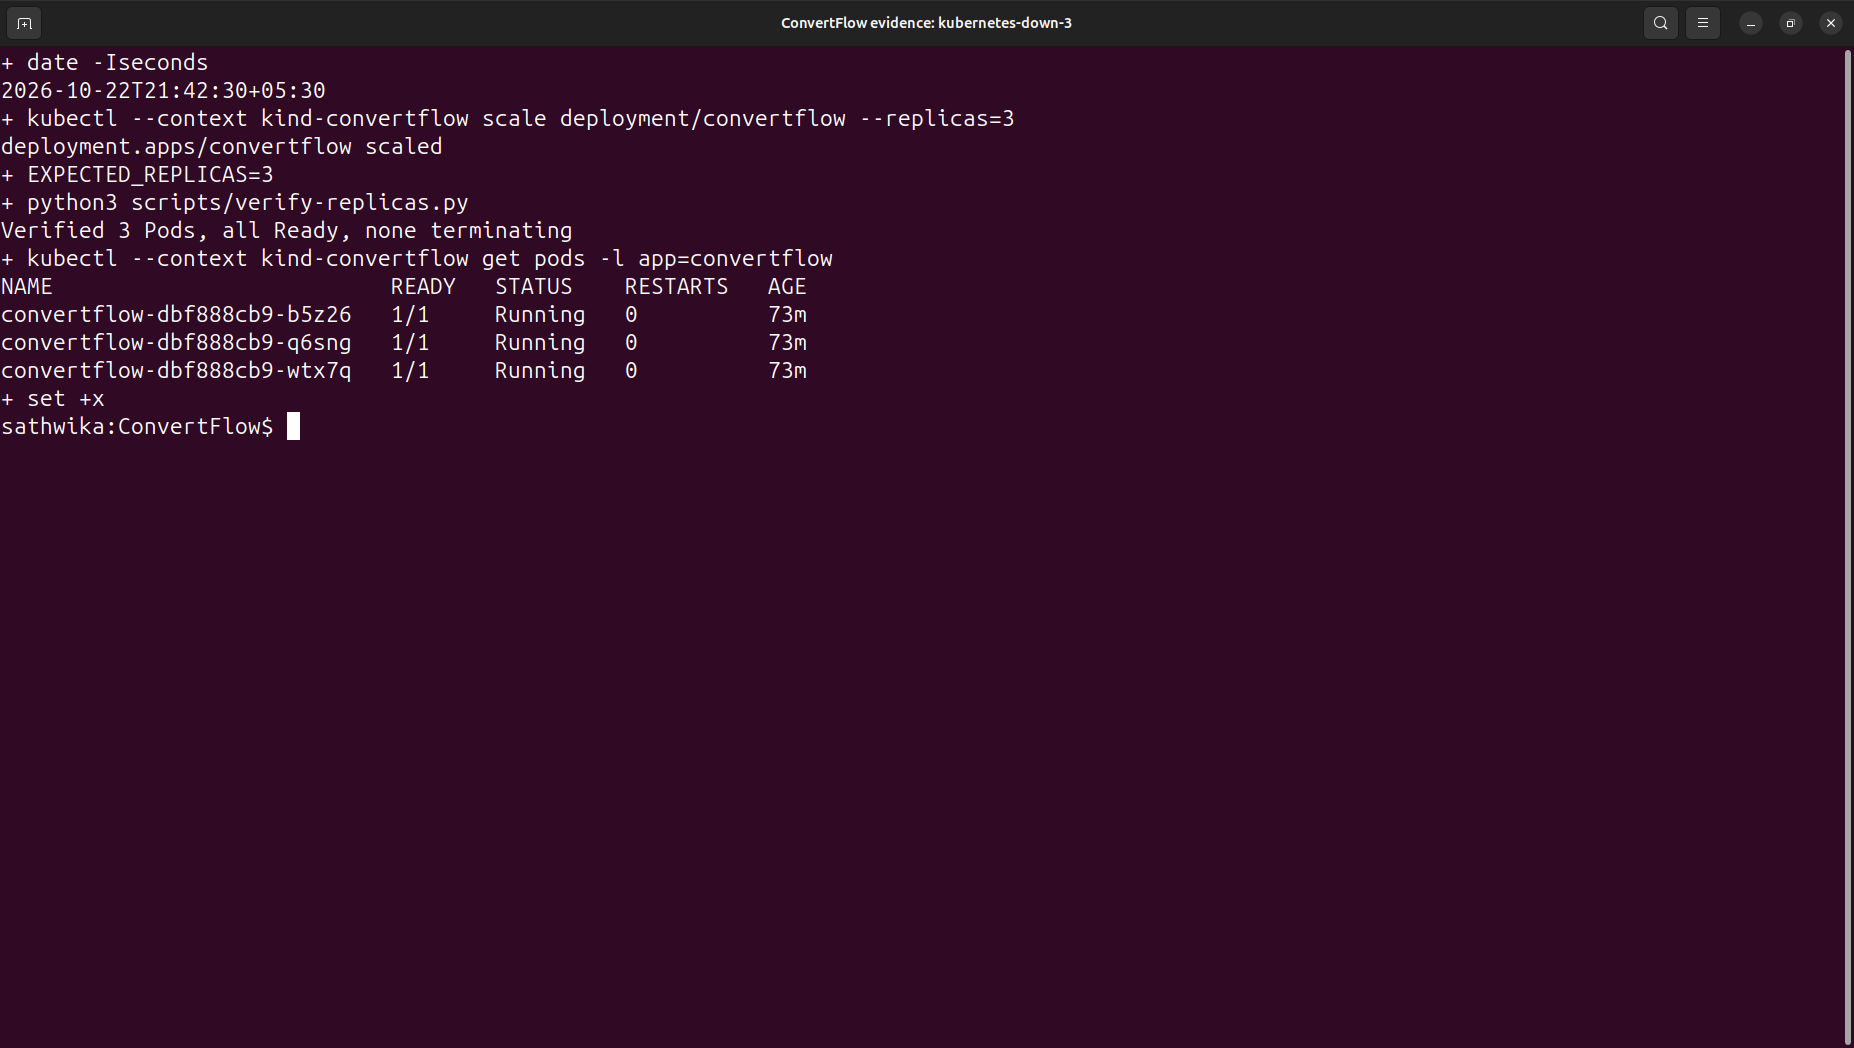
\includegraphics[width=\linewidth,height=0.78\textheight,keepaspectratio]{screenshots/terminal-kubernetes-down-3.png}\end{center}
Figure 18. GNOME Terminal: scale-down command and exact verification of three Ready Pods, with no terminating Pods remaining. Captured 22 Oct 2026, 21:42:37 +0530.
\end{landscape}
\clearpage\begin{landscape}\begin{center}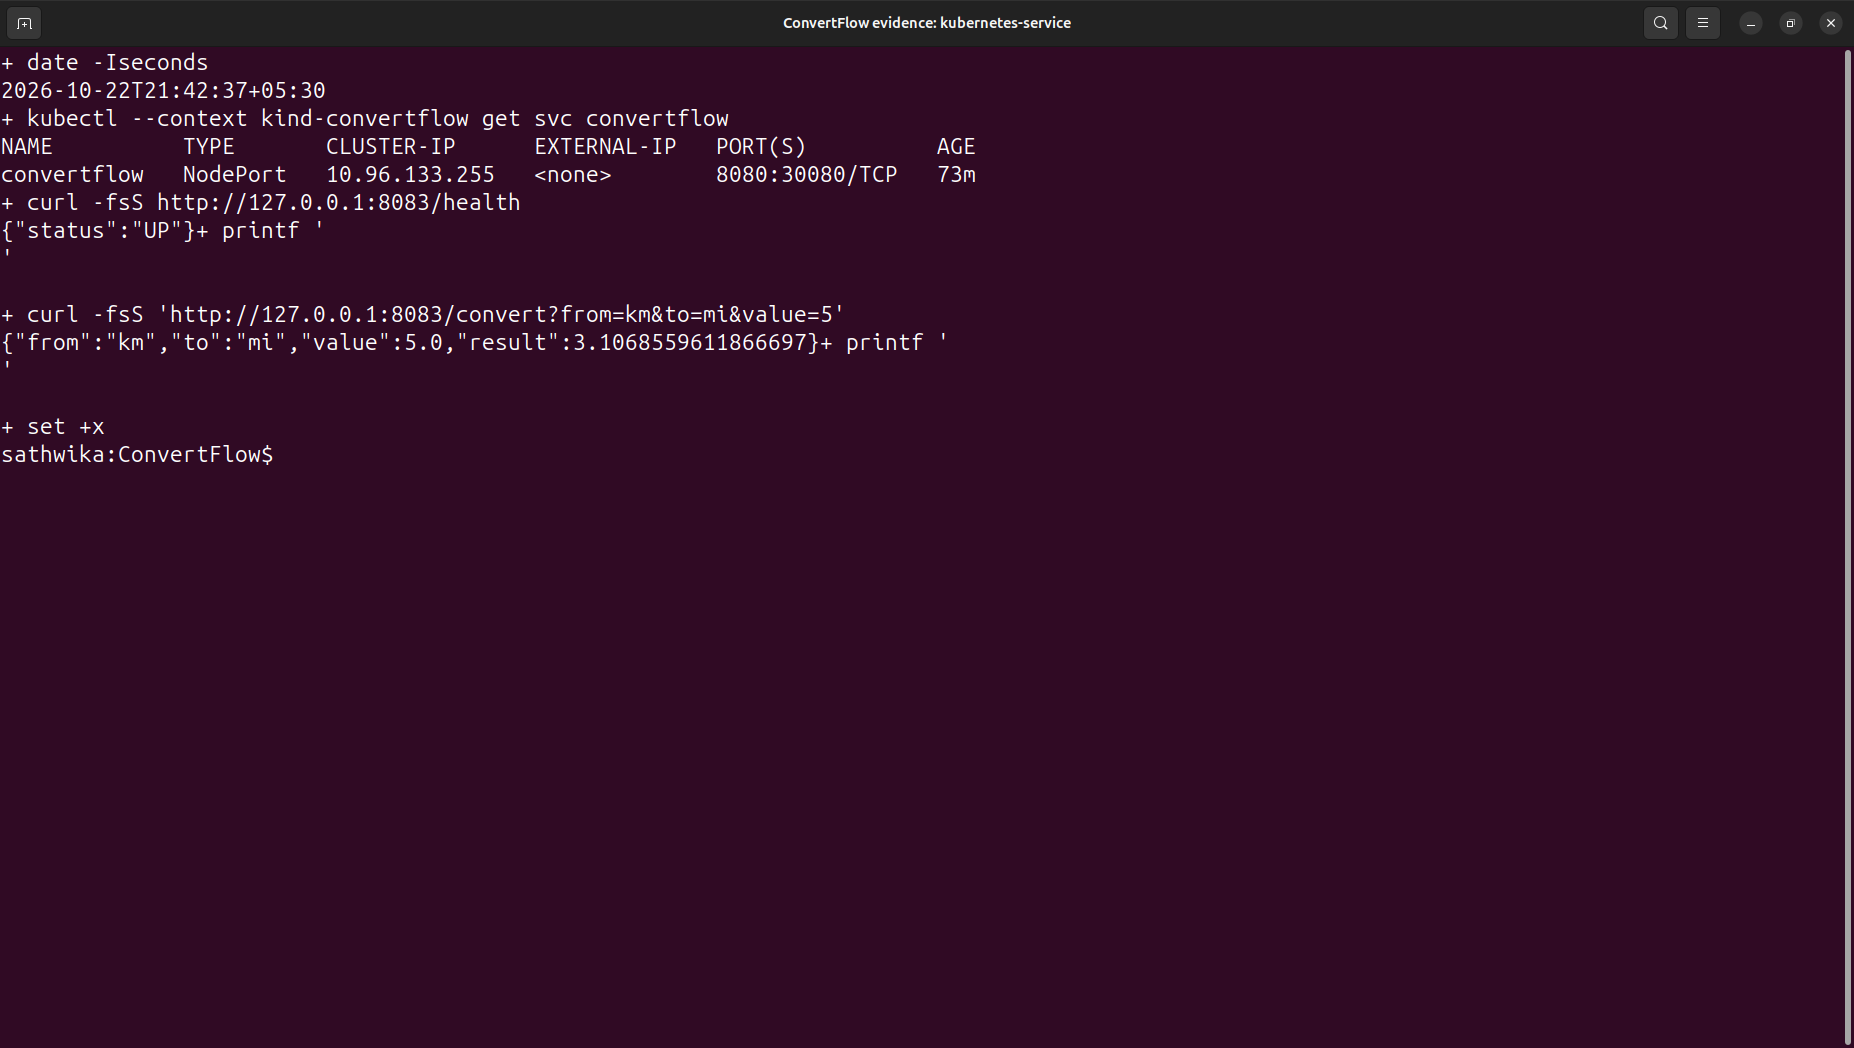
\includegraphics[width=\linewidth,height=0.78\textheight,keepaspectratio]{screenshots/terminal-kubernetes-service.png}\end{center}
Figure 19. GNOME Terminal: actual Service configuration plus health and conversion responses through the Service port-forward on 8083. Captured 22 Oct 2026, 21:42:41 +0530.
\end{landscape}
\clearpage\begin{landscape}\begin{center}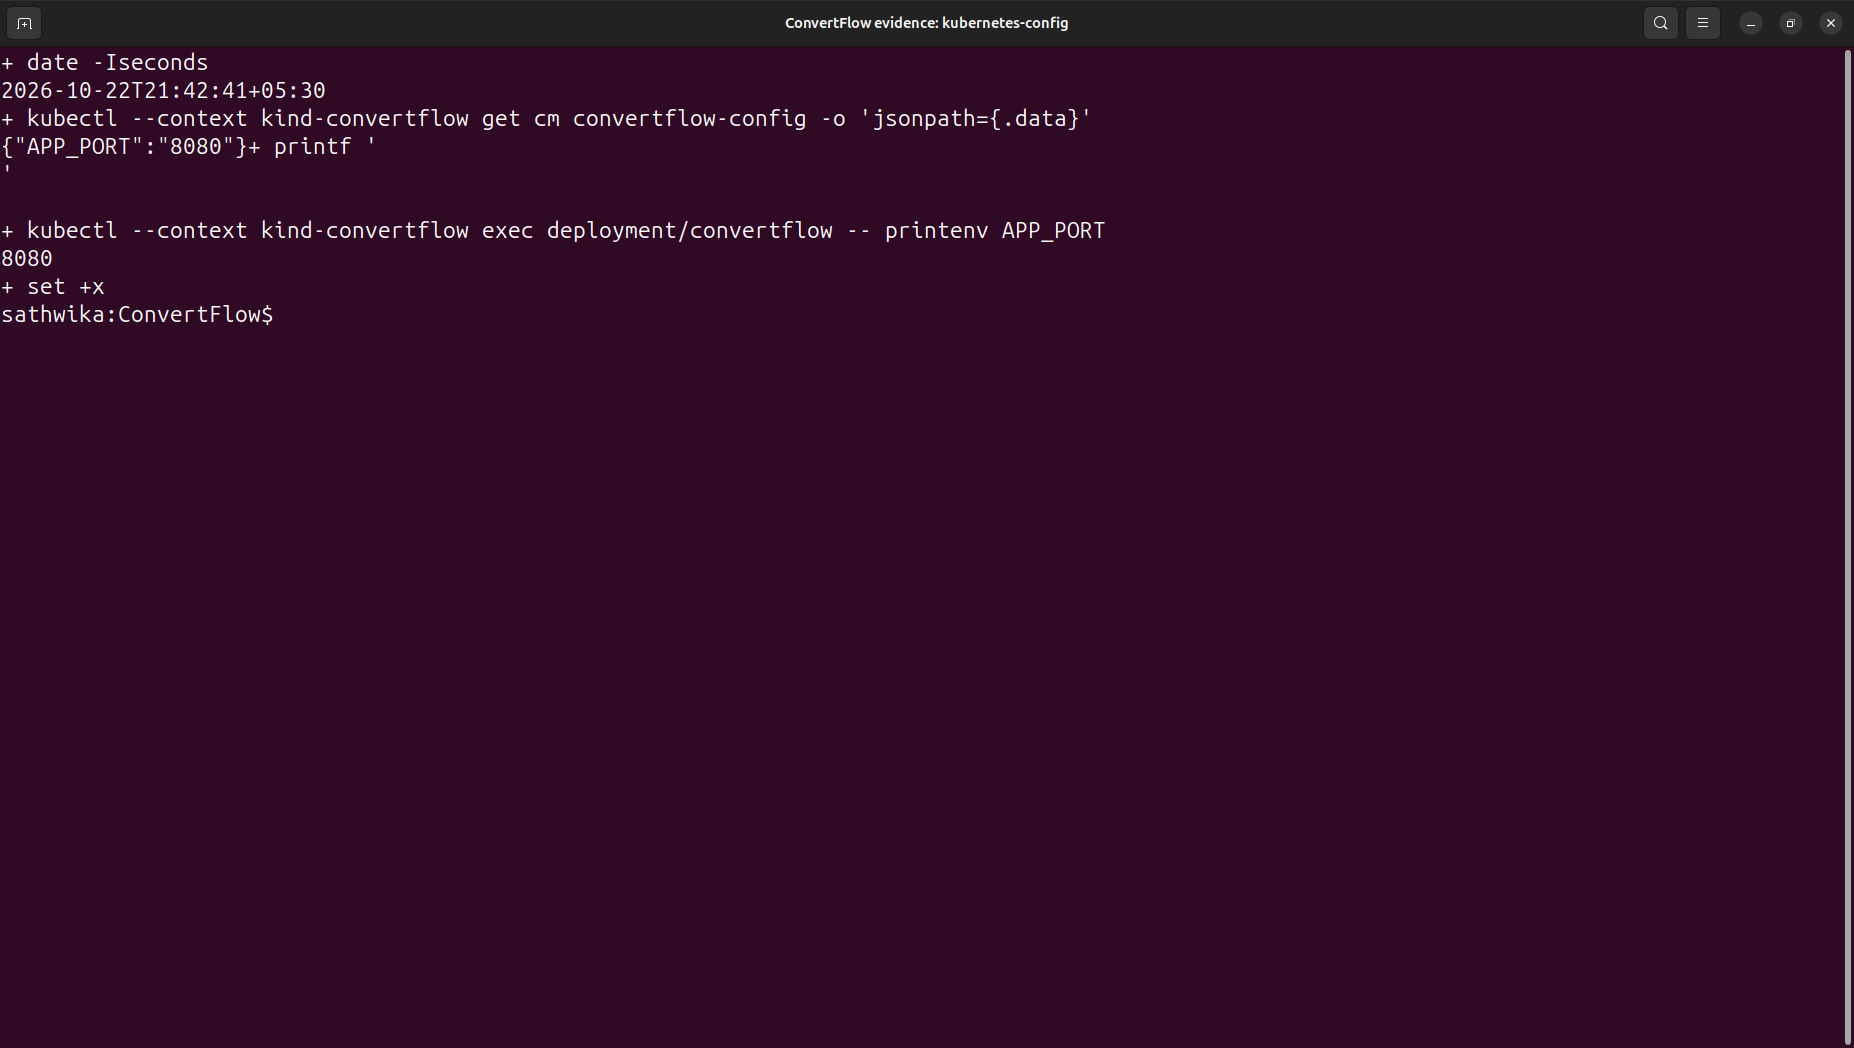
\includegraphics[width=\linewidth,height=0.78\textheight,keepaspectratio]{screenshots/terminal-kubernetes-config.png}\end{center}
Figure 20. GNOME Terminal: ConfigMap APP\_PORT value and printenv inside a running Pod both show 8080, verifying configuration injection. Captured 22 Oct 2026, 21:42:45 +0530.
\end{landscape}
\clearpage\begin{landscape}\begin{center}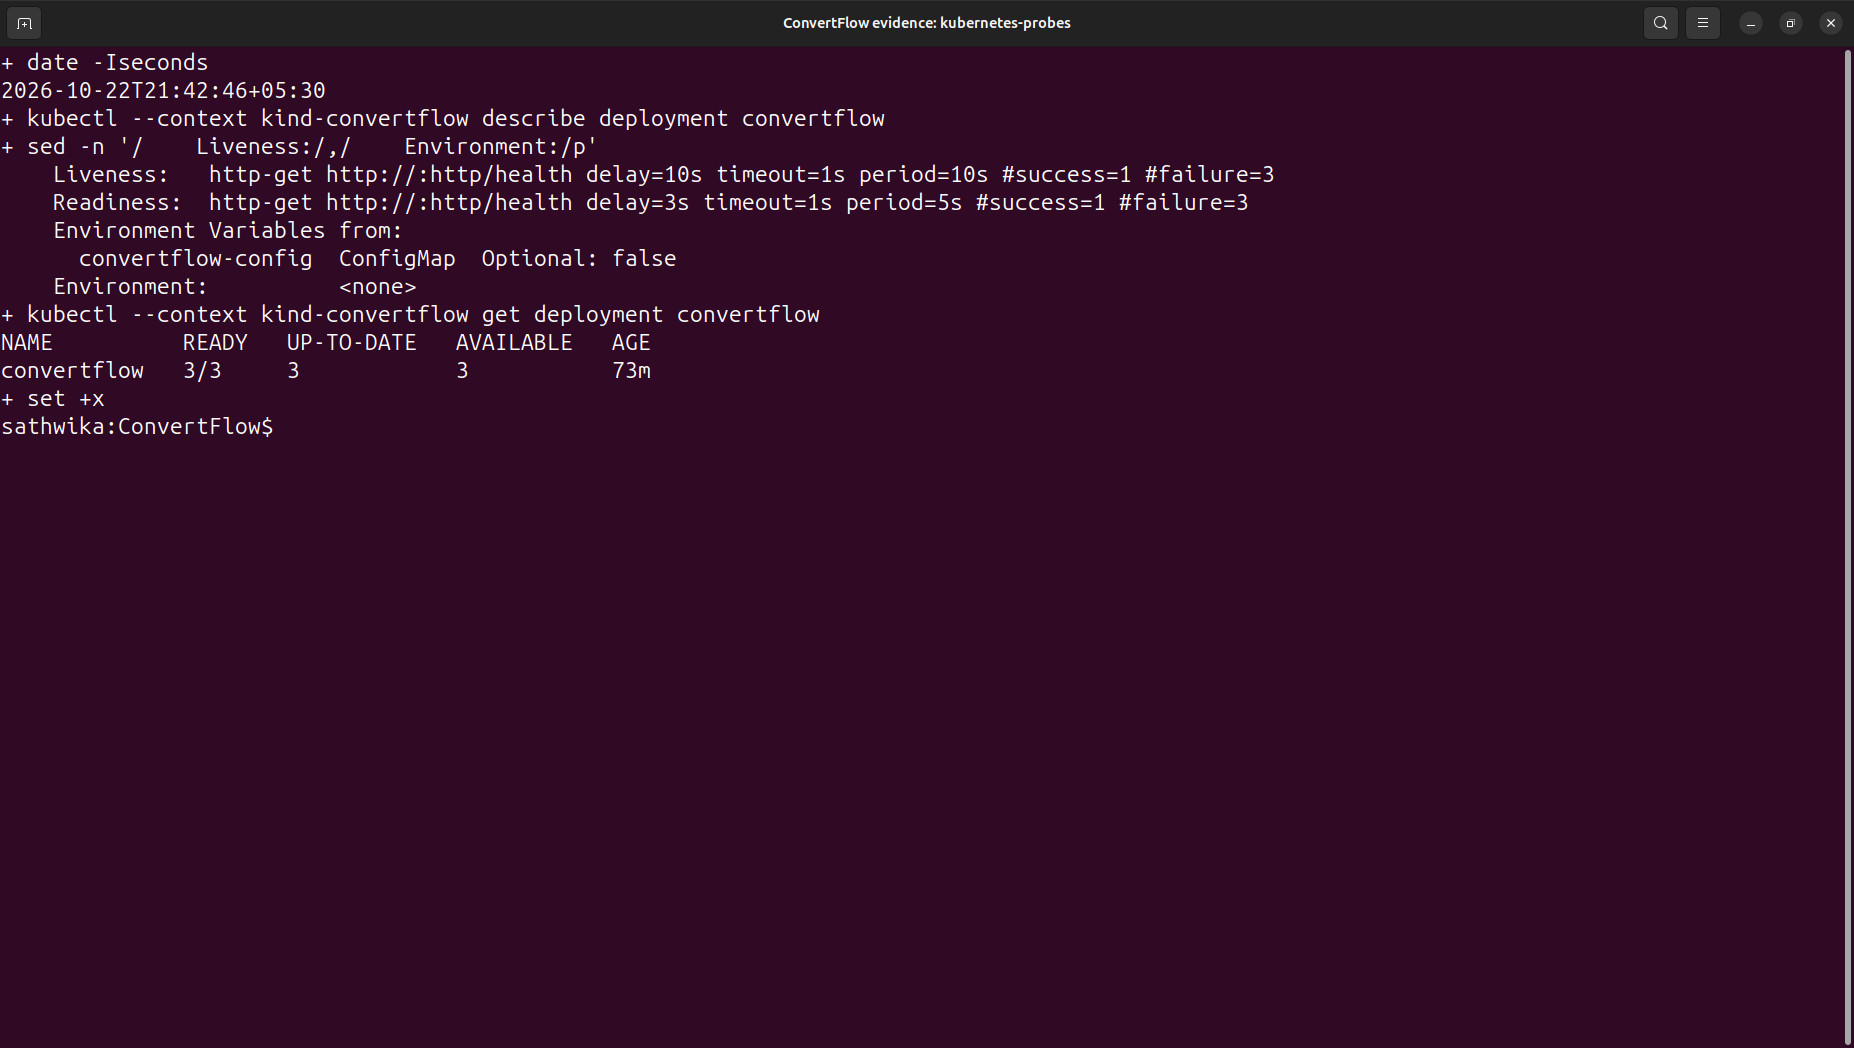
\includegraphics[width=\linewidth,height=0.78\textheight,keepaspectratio]{screenshots/terminal-kubernetes-probes.png}\end{center}
Figure 21. GNOME Terminal: live readiness/liveness probe definitions, ConfigMap reference, and Deployment availability at three replicas. Captured 22 Oct 2026, 21:42:50 +0530.
\end{landscape}
\subsection*{Conclusion}
The same application runs successfully as a systemd service, a Docker container and a Kubernetes workload. Ansible avoids unnecessary changes on the second run; Kubernetes reconciles the requested replica counts while the Service provides a stable access path. The demo remains running, and no cluster, image, container or service cleanup was performed.

\subsection*{References}
Ansible: Handlers: https://docs.ansible.com/projects/ansible/latest/playbook\_guide/playbooks\_handlers.html (accessed 22 October 2026).

Docker: Multi-stage builds: https://docs.docker.com/build/building/multi-stage/ (accessed 22 October 2026).

Kubernetes: Liveness and Readiness Probes: https://kubernetes.io/docs/tasks/configure-pod-container/configure-liveness-readiness-startup-probes/ (accessed 22 October 2026).

Kind: Quick Start: https://kind.sigs.k8s.io/docs/user/quick-start/ (accessed 22 October 2026).

Project repository: https://github.com/1ms24ci042-DS/ConvertFlow (accessed 22 October 2026).

\newpage
\section*{Evidence and submission notes}
The preserved first deployment and Jenkins automatic build \#2 occurred on 22 October 2026. Fresh terminal verification and scaling were also executed on this date; each terminal capture has a timestamped JSON record and an actual session transcript under evidence/terminal/. The historical first Ansible run is reviewed in a terminal and is explicitly distinguished from new execution. All command figures are direct gnome-screenshot captures of GNOME Terminal windows showing executed commands, output and prompts; Jenkins figures remain genuine browser UI captures. No terminal image, successful event or historical timestamp was synthesized. Superseded browser log views, failed focus captures and older rendered illustrations are excluded from the current reports and selected submission figures.

The report uses portrait A4 pages for narrative and individual landscape A4 evidence pages to keep terminal text and Jenkins details readable. Body text and headings are black; screenshots retain their original colours. Page numbering continues across orientations.

The supplied institutional original\_template.tex defines the report structure and assessment rubric. A separate original assignment PDF was not found locally; the pre-existing ConvertFlow\_Report.pdf was an earlier report. The two components each include Abstract, Introduction, Implementation, Enhancement with rationale, Results, Conclusion and References. Signatures and marks remain blank. No coordinator collaborator invitation is required, as instructed by the student.

Repository: https://github.com/1ms24ci042-DS/ConvertFlow. The repository is private, so the evaluator needs authorized access or the clean submission ZIP. Credentials, dependency caches, bundled JDKs and unrelated files are excluded. The working repository and its full history are retained; the ZIP includes a Git bundle for history review and restore.

Archived automatic-build JAR SHA-256: 49264dd38ba335ecfcb0670cbf84a72c89b5096ecc93f591c627047b88112eaf

Live entry points: systemd http://localhost:8080/health; Docker http://localhost:8081/health; Jenkins http://localhost:8082/job/ConvertFlow/; Kubernetes http://localhost:8083/health. The port-forward and Jenkins WAR processes need restarting after reboot. The systemd service and Docker daemon are enabled. Full reproduction details are in README.md and the submitted scripts.

\end{document}
